%\documentclass[11pt,]{article}
%\documentclass[12pt,a4paper]{article}
\documentclass[11pt,a4paper]{article}
\usepackage[T1]{fontenc}
\usepackage{lmodern}
\usepackage{amssymb,amsmath}
\usepackage{ifxetex,ifluatex}

\RequirePackage[utf8]{inputenc} 
%\RequirePackage[T1]{fontenc}
%\usepackage[english,francais]{babel}
\usepackage[english]{babel}
%\usepackage[pdftex]{hyperref}	
\usepackage[Brest,version]{telecom}	
\usepackage{aeguill}
\usepackage{times}
\usepackage{listingsutf8}

\usepackage{fixltx2e} % provides \textsubscript
% Set line spacing
% use upquote if available, for straight quotes in verbatim environments
\IfFileExists{upquote.sty}{\usepackage{upquote}}{}
\ifnum 0\ifxetex 1\fi\ifluatex 1\fi=0 % if pdftex
  \usepackage[utf8]{inputenc}
\else % if luatex or xelatex
  \ifxetex
    \usepackage{mathspec}
    \usepackage{xltxtra,xunicode}
  \else
    \usepackage{fontspec}
  \fi
  \defaultfontfeatures{Mapping=tex-text,Scale=MatchLowercase}
  \newcommand{\euro}{€}
\fi
% use microtype if available
\IfFileExists{microtype.sty}{\usepackage{microtype}}{}
%\usepackage[margin=1in]{geometry}
\usepackage{longtable,booktabs}
\usepackage{graphicx}
% Redefine \includegraphics so that, unless explicit options are
% given, the image width will not exceed the width of the page.
% Images get their normal width if they fit onto the page, but
% are scaled down if they would overflow the margins.
\makeatletter
\def\ScaleIfNeeded{%
  \ifdim\Gin@nat@width>\linewidth
    \linewidth
  \else
    \Gin@nat@width
  \fi
}
\makeatother
\let\Oldincludegraphics\includegraphics
{%
 \catcode`\@=11\relax%
 \gdef\includegraphics{\@ifnextchar[{\Oldincludegraphics}{\Oldincludegraphics[width=\ScaleIfNeeded]}}%
}%
\ifxetex
  \usepackage[setpagesize=false, % page size defined by xetex
              unicode=false, % unicode breaks when used with xetex
              xetex]{hyperref}
\else
  \usepackage[unicode=true]{hyperref}
\fi
\hypersetup{breaklinks=true,
            bookmarks=true,
            pdfauthor={Lisa MALIPHOL},
            pdftitle={diateam SCAD@COPS A Hybrid Network Intrusion Detection System},
            colorlinks=true,
            citecolor=blue,
            urlcolor=blue,
            linkcolor=magenta,
            pdfborder={0 0 0}}
\urlstyle{same}  % don't use monospace font for urls
\setlength{\parindent}{0pt}
\setlength{\parskip}{6pt plus 2pt minus 1pt}
\setlength{\emergencystretch}{3em}  % prevent overfull lines
\setcounter{secnumdepth}{5}



%%% Change title format to be more compact
\usepackage{titling}
\setlength{\droptitle}{-2em}
  \title{diateam\\SCAD@COPS\\A Hybrid Network Intrusion Detection System}
  \pretitle{\vspace{\droptitle}\centering\huge}
  \posttitle{\par}
  \author{Lisa MALIPHOL}
  \preauthor{\centering\large\emph}
  \postauthor{\par}
  \date{}
  \predate{}\postdate{}

\version{1.0}													% version du document, avec option version
\docdescription{A Hybrid Network Intrusion Detection System}


\begin{document}

\TBfrontcover

\thispagestyle{empty}

\newpage
\thispagestyle{empty} \mbox{}

\clearpage

\maketitle


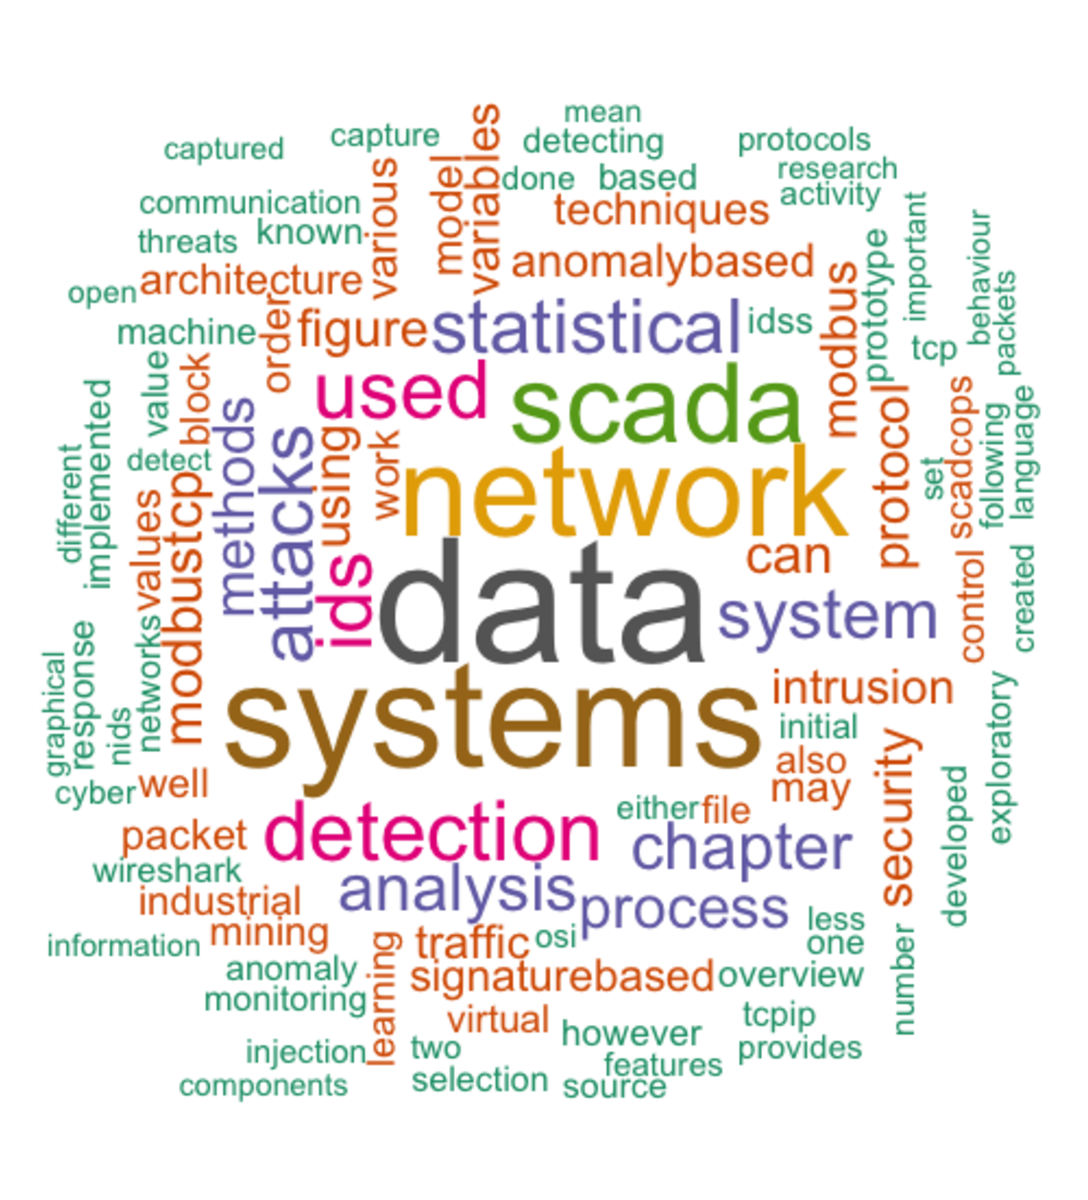
\includegraphics{thesis_files/figure-latex/unnamed-chunk-3-1.pdf}

\thispagestyle{empty}

\newpage
\thispagestyle{empty} \mbox{}

\clearpage
\pagenumbering{roman}

\begin{center}

\vspace{30mm}

{\Huge diateam}\\
\bigskip
{\Huge SCAD@COPS}\\
\bigskip
\bigskip
{\Huge A Hybrid}\\
{\Huge Network Intrusion Detection System}\\
\vspace{15mm}
{\Large by}\\
\vspace{10mm}
{\huge Lisa MALIPHOL}\\

\vspace{25mm}

\textit{A thesis submitted in partial satisfaction of the}\\
\medskip
\textit{requirements for the diploma of the}\\
\medskip
\textit{Masters of Science}\\
\medskip
\textit{in}\\
\medskip
\textit{Computer Science and Decision Systems}\\
\medskip
\textit{in the}\\
\medskip
\textit{Grande École}\\
\medskip
\textbf{\textit{\Large Télécom Bretagne}}\\

\vspace{15mm}

Corporate Advisor:\\
\smallskip
Guillaume Prigent\\
\bigskip
\medskip
Academic Advisors:\\
\smallskip
Professor Yannis Haralambous\\
Professor Sandrine Vaton\\

\vspace{15mm}

\textit{September 2015}\\
\medskip
\textit{Plouzané, FRANCE}\\

\end{center}

\thispagestyle{empty} \newpage
\mbox{} \thispagestyle{empty}

\newpage

\begin{center}

\vspace{30mm}

{\Huge diateam}\\
\bigskip
{\Huge SCAD@COPS}\\
\bigskip
\bigskip
{\Huge Un système hybride de détection}\\
{\Huge d’intrusion de réseau }\\

\vspace{30mm}
{\huge Lisa MALIPHOL}\\

\vspace{75mm}
\textit{septembre 2015}\\
\medskip
\textit{Plouzané, FRANCE}\\

\end{center}

\thispagestyle{empty} \newpage
\mbox{} \thispagestyle{empty}

\newpage

\section*{Acknowledgements}\label{acknowledgements}
\addcontentsline{toc}{section}{Acknowledgements}

\newpage
\mbox{} \thispagestyle{empty}

\clearpage

\section*{Abstract}\label{abstract}
\addcontentsline{toc}{section}{Abstract}

Large scale, industrial processes and infrastructure, such as in the
energy, or manufacturing sectors, may span across multiple, large,
remote and disconnected geographical areas and are comprised of multiple
devices, controllers and sensors. They are managed, monitored and
controlled by computer systems called Supervisory Control and Data
Acquisition (SCADA) systems. Previously, these systems resided on their
own networks and used proprietary protocols and software, and therefore
through obscurity and isolation were moderately immune to outside
threats. Over time, with the advancement of technologies, such as in
computing systems and networking, and increased interconnectivity to
traditional IT systems they have become susceptible and more vulnerable
to cyber attacks.

In order to address this issue, Network Intrusion Detection Systems
(NIDS) have been put in place in SCADA environments to monitor and
survey the network and systems to identify suspicious, or anomalous
activities and events. Signature-based NIDSs are an established method
previously utilized, although anomaly-based NIDS have grown in interest.
In contrast to signature-based methods, which are very capable and more
accurate in identifying known attacks, anomaly-based NIDSs are appealing
as they can detect novel, never seen before attacks. Anomaly-based
approaches may be based on statistical, data mining, or machine learning
methods.

diateam has proposed a hybrid network intrusion detection system that
not only provides measures in better securing the device itself, but
more importantly, combines both signature- and anomaly-based techniques.
The inception of the hybrid NIDS is the proof of concept that is
presented in this paper. This study also incorporates another diateam
product, the Virtual Scada Box, as the testbed for conducting analysis
and evaluation as real-world network attack data is generally
restricted.

\bigskip
\bigskip
\textbf{Keywords: } NIDS, Anomaly-based Network Intrusion Detection,
Industrial Control Systems, SCADA Systems, MODBUS/TCP

\newpage
\mbox{} \thispagestyle{empty}

\clearpage

\section*{Résumé}\label{resume}
\addcontentsline{toc}{section}{Résumé}

Les sites industriels importants, telle qu'on en trouve dans le secteur
de l'énergie, sont composés de multiples centres de productions pouvant
être éloignés géographiquement les uns des autres. Ces différents sites
sont reliés par de nombreux canaux de communication par lesquels passent
des informations de contrôle et de commande de la production. L'ensemble
de ce réseau est communément appelé par l'acronyme anglais SCADA
``Supervisory Control and Data Acquisition'' qui peut être traduit en
français par: système de contrôle et d'acquisition de donnée.

Auparavant, ces systèmes résidaient sur leur propres réseaux et
utilisaient des protocoles et logicielles propriétaires. Leur isolation
du réseau ainsi que la méconnaissance de leur protocoles les rendait
relativement à l'abri de menaces extérieures. Au fil du temps, avec
l'évolution des technologies, notamment des systèmes informatiques et
des réseaux , ainsi que l'augmentation de l'interconnectivité avec des
systèmes informatiques traditionnels, les ont rendu sensibles et
vulnérables face aux attaques informatiques.

Afin de faire face à ces enjeux, les systèmes de détection d'intrusion
réseau (NIDS) ont été mis en place dans des environnements SCADA pour
surveiller les réseaux et les systèmes. Cela afin d'identifier les
activités et les événements suspects ou anormaux. Actuellement la
majorité des NIDS se basent sur une liste de signatures, mais de plus en
plus on s'orientent vers des mécanismes de détection d'anomalies.
Contrairement aux systèmes basées sur des signatures qui sont très
efficace et plus précis dans l'identification des attaques connues, les
NIDS basées sur des anomalies sont attrayant car ils peuvent détecter
des nouvelles attaques qui n'ont jamais été vu auparavant. Les approches
basées sur des anomalies s'appuient sur des méthodes statistiques, de
fouilles de données, ou de machine learning.

diateam a proposé an système hybride de détection d'intrusion qui
fournit non seulement des mesures pour protéger le dispositif lui-même,
mais surtout, combine les deux techniques basées sur des signatures et
des anomalies. C'est ce NIDS hybride, développé comme une preuve de
concept, qui sera présenté dans ce document. Ce rapport décrira
également un autre produit de diateam, la boîte SCADA virtuel, qui sert
de banc d'essai pour la réalisation d'analyses et d'évaluation. Ainsi
diateam garde la maîtrise sur la détection et l'analyse des données
d'attaques, celles-ci étant généralement confidentielles.

\bigskip
\bigskip
\textbf{Mots-clés: } détection d'intrusion réseau (NIDS), détection
d'intrusion basée sur des anomalies, systèmes industriels, systèmes de
contrôle et d'acquisition de données (SCADA), MODBUS/TCP

\newpage
\mbox{} \thispagestyle{empty}

\clearpage

\section*{diateam}\label{diateam}
\addcontentsline{toc}{section}{diateam}

diateam is a small-medium sized enterprise located in Brest, FRANCE.
They cover a wide range of services in information systems, software
development, as well as cybersecurity. diateam's R\&D group utilizes the
latest in technologies in its projects. Their solutions have been
implemented by the French Ministry of Defense, public and private
companies, in addition to the higher educational system by means of the
cybersecurity trainings offered.

As a Data Scientist Intern at diateam, the following work was
accomplished during the end-of-studies internship required for the
Masters of Science diploma at Télécom Bretagne.

\newpage
\mbox{} \thispagestyle{empty}

\clearpage

\tableofcontents

\cleardoublepage

\listoffigures

\cleardoublepage

\listoftables

\newpage

\section*{Acronyms}\label{acronyms}
\addcontentsline{toc}{section}{Acronyms}

\begin{longtable}[c]{@{}rl@{}}
\toprule\addlinespace
A-NIDS & Anomaly-based Network Intrusion Detection System
\\\addlinespace
DARPA & Defense Advanced Research Project Agency
\\\addlinespace
EDA & Exploratory Data Analysis
\\\addlinespace
HMI & Human-Machine Interface
\\\addlinespace
HNS & Hybrid Network Simulation
\\\addlinespace
ICS & Industrial Control System
\\\addlinespace
IDS & Intrusion Detection System
\\\addlinespace
IPS & Intrusion Prevention System
\\\addlinespace
MTU & Master Terminal Unit
\\\addlinespace
NIDS & Network Intrusion Detection System
\\\addlinespace
OSI & Open Standards Interconnection
\\\addlinespace
PLC & Programmable Logic Controller
\\\addlinespace
POC & Proof of Concept
\\\addlinespace
RTU & Remote Terminal Unit
\\\addlinespace
SCADA & Supervisory Control and Data Acquisition
\\\addlinespace
TCP/IP & Transmission Control Protocol/Internet Protocol
\\\addlinespace
\bottomrule
\end{longtable}

\newpage
\mbox{} \thispagestyle{empty}

\clearpage
\pagenumbering{arabic}

\setcounter{page}{17}

\section{Introduction}\label{introduction}

Supervisory Control and Data Acquisition Systems (SCADA) are one type of
industrial control systems put in place for monitoring and controlling
industrial processes, such as those in the energy or manufacturing
sectors. Originally, these systems were isolated and used proprietary
protocols, whose security relied predominantly on obscurity. As SCADA
systems have moved towards open standards and have become more
interconnected to traditional information technology systems, these
critical systems have also become increasingly exposed and targeted to
cyber attacks.{[}1, 2{]}

In order to address the growing concern of the vulnerability of SCADA
systems, Intrusion Detection Systems (IDS) are progressively being put
strategically into place in order to monitor and analyze, and ultimately
alert to devious behaviors. These devices can be either signature-, or
anomaly-based, however, there are trade-offs in terms of accuracy and
robustness between the two types of systems.

A hybrid IDS has been proposed by diateam under the project name
SCAD@COPS. The aim of the work presented in this paper was to realize
the anomaly-based component of this Proof of Concept (POC). Based on the
contributions of {[}3{]} and {[}4{]}, the POC integrates the
architectural and signature-based aspects as described in their work,
and where the following constraints were taken into consideration in its
design -- network-based and passive only; the IDS should not interfere
with, nor modify the SCADA system; and only TCP/IP data are analyzed.

This work began with an in-depth research of SCADA systems, related
subject matter, IDSs and the state of the art of its application to
SCADA systems, in addition to the methods of anomaly detection. Then, an
exploratory analysis of the data was done, which preceded the
implementation of the initial POC based on statistical metrics.

As such, this paper is organized and divided into the following major
sections:

\begin{itemize}
\itemsep1pt\parskip0pt\parsep0pt
\item
  Chapter 1 gives an introduction to this work, and outlines its
  organization
\item
  Chapter 2 provides an overview of SCADA systems
\item
  Chapter 3 provides some basic networking principles
\item
  Chapter 4 briefly considers a few common cyber attacks
\item
  Chapter 5 discusses intrusion detection systems
\item
  Chapter 6 summarizes different approaches for detecting network
  intrusions
\item
  Chapter 7 describes the data source analyzed
\item
  Chapter 8 gives an overview of the exploratory data analysis
\item
  Chapter 9 describes the architecture and implementation of the proof
  of concept
\item
  Chapter 10 outlines the statistical measures and features applied
\item
  Chapter 11 describes the testing and evaluation process
\item
  Chapter 12 summarizes and concludes
\end{itemize}

\clearpage

\section{Overview of SCADA Systems}\label{overview-of-scada-systems}

\subsection{ICS}\label{ics}

An Industrial Control System (ICS) comprises such systems as Supervisory
Controls and Data Acquisition (SCADA), Distributed Control Systems
(DCS), and smaller systems such as Programmable Logic Controllers (PLC)
that are control systems predominantly used in industrial production.

ICSs were initially developed to meet the requirements of performance,
reliability, safety and flexibility. They existed prior to the
advancement in computer and network technology, such as public and
private networks, desktop computing, or the Internet. Since ICSs
remained rather isolated and obscure, the dangers of cyber security were
less, or non-existent.

Typically, industrial control systems are continuously operational and
commonly serve vital public services and infrastructure, thus preventive
security measures must be put into place. The compromise of SCADA
systems may have negative consequences including, but not limited to,
substantial damage to the environment, significant risk to human safety
and health, and financial and production losses.

\subsection{SCADA}\label{scada}

A Supervisory Control and Data Acquisition system is an ICS used for
monitoring equipment and controlling processes in industries such as
electrical, water, oil and manufacturing. The administration over a
geographically widely distributed process can be directed from a central
location at the Master Terminal Unit (MTU) in SCADA systems. Changes to
process controllers, the opening and closing of valves and switches, the
monitoring and the measurement of information is administered from the
MTU to Remote Terminal Units (RTU). Due to their economy, versatility,
flexibility, and configurability, programmable logic controllers, which
are small industrial field devices are widely used as RTUs.{[}5{]} The
various components of a SCADA system is shown (Figure 1).{[}1{]}

Additionally, SCADA systems commonly include PLCs, small industrial
computers made to perform logic functions executed by electrical
hardware, which control sensors and actuators. Human operators modify
control settings, override automatic processes manually, and monitor the
state of the processes under control via an Human Interface Control
(HMI). It is from these HMIs that the PLCs are managed.

These systems have differing constraints and properties from those of
traditional IT systems, the most prominent being that they are real-time
operational systems that must always be available and run continuously
without outage. Once the field devices have been put into place, they
are normally left untouched, i.e., not rebooted, and left running for
years. This creates the problem of the systems being more susceptible to
buffer overflow due to the accumulation of fragmentation.{[}2{]}

Historically, SCADA systems resided on their own internal networks and
were not connected to other networks. They implemented proprietary
protocols and were, therefore, less vulnerable to network attacks.
However, over time as these systems adopted open standards and leveraged
traditional enterprise systems to lower costs, to increase functionality
and productivity, SCADA systems are also now increasingly exposed to
internal and external attacks.

\begin{figure}

{\centering 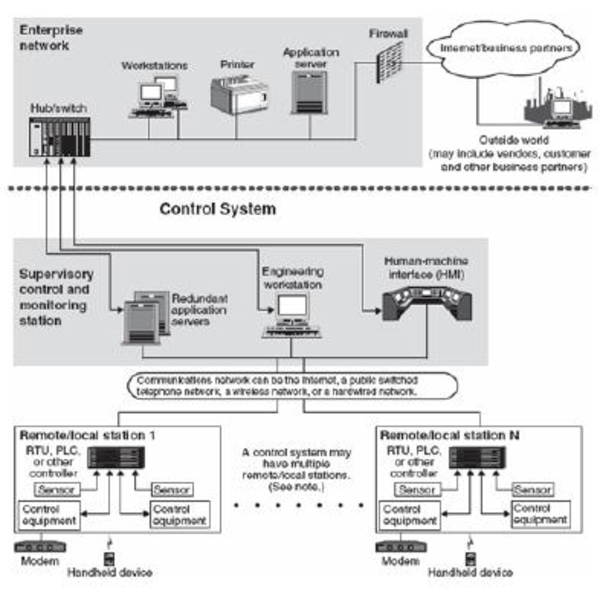
\includegraphics{thesis_files/figure-latex/unnamed-chunk-4-1} 

}

\caption{SCADA components}\label{fig:unnamed-chunk-4}
\end{figure}

\subsection{Traffic characterization}\label{traffic-characterization}

As seen in the comparative analysis done in {[}6{]}, it is shown how the
traffic greatly differs between SCADA and traditional networks. Most
traffic is generated by automated processes in SCADA networks as opposed
to human-generated traffic predominant in traditional networks. The
traffic pattern generated in SCADA networks have been found to be fairly
static and repetitive, with its network topology unchanging, or rarely
modified. Likewise, it is usual for there to be a limited number of
applications and protocols that run on industrial systems.{[}7{]}
Considerably seen over MODBUS traffic, the messages exchanged between
PLCs are recurrent giving it a fixed pattern and relatively stationary
process.{[}8--10{]}

\clearpage

\section{Networking Overview}\label{networking-overview}

In this section, a few fundamental networking terms are discussed.
First, an outline of the OSI model is described, followed by the TCP/IP
and MODBUS protocols.

\subsection{OSI}\label{osi}

Known as the Open System Interconnection (OSI) model, it was initially
developed by the International Standards Organization (ISO) to define
and characterize the communication between computing systems. The OSI
model, as shown in Figure 2
(\href{https://engineering.linkedin.com/endorsements/geographic-trends-skills-using-linkedins-endorsement-feature}{Image
source}) is represented as layers, each one expressed as a protocol.
Each layer serves the layer above it, and the lowest one being closest
to the physical medium carrying the communication. Figure 2 depicts each
layer and its role and responsibilities.

\subsection{Protocols}\label{protocols}

As SCADA systems have become increasingly interconnected to enterprise
networks, they have started to leverage and operate over more modern
protocols. Numerous vendors, such as Schneider, Sew and Siemens,
manufacture programmable logic controllers. Depending on the device, or
manufacturer, PLCs may use a proprietary protocol, such as the Siemens
SIMATIC S7-300. In most cases, however, the MODBUS protocol has been
widely adopted and is predominantly supported by many SCADA network
appliances. As such, this work focuses primarily on examining the
MODBUS/TCP protocol.

\begin{figure}[h]

{\centering 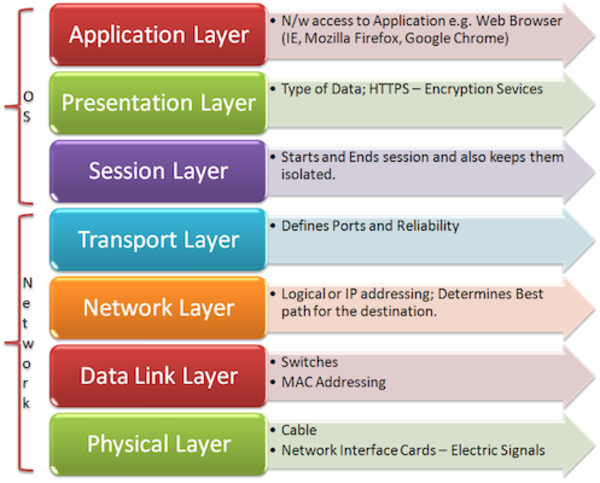
\includegraphics{thesis_files/figure-latex/unnamed-chunk-5-1} 

}

\caption{OSI Model}\label{fig:unnamed-chunk-5}
\end{figure}

\subsubsection{Transmission Control Protocol/Internet Protocol
(TCP/IP)}\label{transmission-control-protocolinternet-protocol-tcpip}

Initially developed by the Defense Advanced Research Project Agency
(DARPA) in the late 1960s, the Internet protocol suite was the result of
the research and development of data transmission technologies in the
United States that was utilized as a standard for military computer
networking.

TCP/IP provides reliable, ordered and error-checked delivery of streams
of octets between applications running on hosts communicating over an IP
network. A detailed illustration of the IP and TCP headers can be seen
in Figures 3
(\href{http://nmap.org/book/images/hdr/MJB-TCP-Header}{Image credit: Max
Baxter}) and Figure 4
(\href{http://nmap.org/book/images/hdr/MJB-IP-Header}{Image credit: Max
Baxter}).

\begin{figure}[h]

{\centering 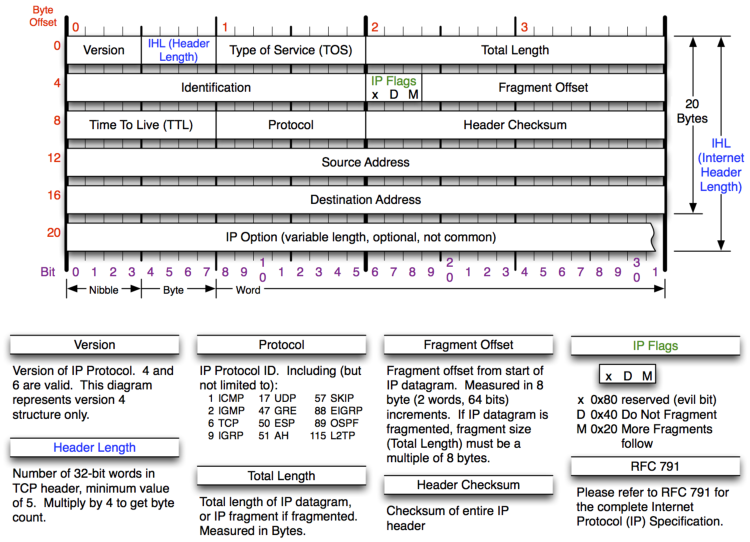
\includegraphics{thesis_files/figure-latex/unnamed-chunk-6-1} 

}

\caption{IPv4 Header}\label{fig:unnamed-chunk-6}
\end{figure}

\begin{figure}[h]

{\centering 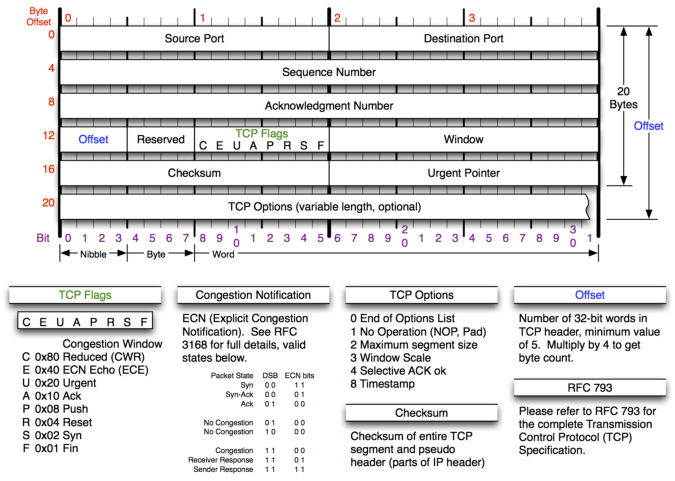
\includegraphics{thesis_files/figure-latex/unnamed-chunk-7-1} 

}

\caption{TCP Header}\label{fig:unnamed-chunk-7}
\end{figure}

\subsubsection{MODBUS Protocol}\label{modbus-protocol}

The MODBUS protocol is an open standard and popular network protocol
implemented in ICS devices that were initially developed over serial
communication, then later adapted for TCP/IP. It is a request/reply
messaging protocol located at the application layer that was created to
communicate with PLCs in industrial systems. However, due to the limited
resources that PLCs have, it was designed to be a simple protocol that
provides no security against unauthorized commands or interception of
data.{[}11{]}. Figure 5 gives an example architecture for MODBUS TCP
communication.

\begin{figure}[h]

{\centering 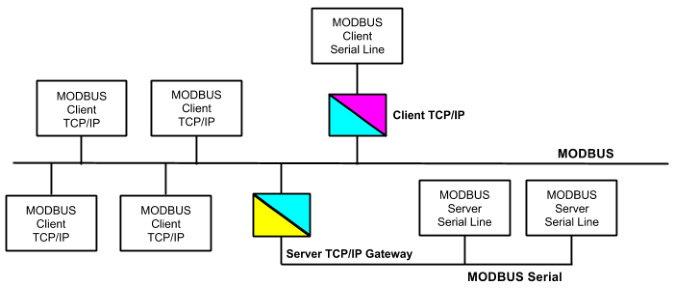
\includegraphics{thesis_files/figure-latex/unnamed-chunk-8-1} 

}

\caption{MODBUS TCP/IP Communication Architecture}\label{fig:unnamed-chunk-8}
\end{figure}

The master initiates a request and the slave sends a response containing
either data or error. The common implementations of MODBUS are over
Ethernet networks (MODBUS/TCP) or Serial buses (MODBUS/RTU). Both forms
of MODBUS contain the Packet Data Unit (PDU), the component consisting
of a function code and data that is independent of the communication
layer.

Attached to the PDU is the application specific addressing and error
checking, which together comprise the Application Data Unit (ADU). In
MODBUS/TCP, the ADU is encapsulated in the TCP packet, so error checking
is omitted from the MODBUS/TCP ADU, because it is already provided in
the TCP layer (Figure 6).

\begin{figure}[h]

{\centering 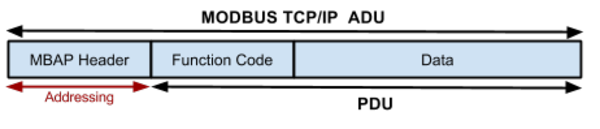
\includegraphics{thesis_files/figure-latex/unnamed-chunk-9-1} 

}

\caption{MODBUS/TCP Frame}\label{fig:unnamed-chunk-9}
\end{figure}

Included in the MODBUS Application Protocol (MBAP) are:

\begin{itemize}
\itemsep1pt\parskip0pt\parsep0pt
\item
  Transaction ID - 2 bytes - identifies request/response pairs
\item
  Protocol ID - 2 bytes - is always 00 00 for MODBUS protocol
\item
  Length - 2 bytes - identifies the number of bytes in the following
  message
\item
  Unit ID - 1 byte - used to distinguish which slave is addressed when
  several slaves use the same IP address
\end{itemize}

In MODBUS/TCP, port 502 is typically the default port reserved for
MODBUS communication. Furthermore, when identifying MODBUS requests, the
services specified are indicated by the MODBUS function code. Appendix A
lists the public function codes available.

With no authentication and authorization mechanisms, data integrity
checks, or encryption due to the simple design of the MODBUS protocol,
SCADA network components do not verify identity or permissions,
determine legitimacy of message content, nor provide confidentiality.

\clearpage

\section{Common Attacks on SCADA}\label{common-attacks-on-scada}

{[}5, 12--15{]} define threats and vulnerabilities, security issues, as
well as policies and best practices, and recommendations on how to best
secure SCADA systems. Nonetheless, cyber attacks continue to increase as
SCADA systems become more exposed and as the attacks grow in
sophistication. Due to the private nature of the data, however, little
has been published regarding MODBUS/TCP attacks apart from the work of
Digital Bond\footnote{\url{http://www.digitalbond.com}}.

Leveraging existing enterprise network infrastructure, SCADA systems are
also at risk to the same threats that typical IT systems encounter. In
addition, as SCADA systems are upgraded less frequently and continue to
run on legacy systems, they are rendered even more vulnerable to various
attacks that may be prevented by deploying upgrades that address newer
and known threats. In {[}2{]}, outlines and describes in detail the
various methods of cyber attacks on software and hardware and ways of
compromising SCADA systems.

The following is a non-exhaustive list of of attacks that provides an
overview of just some of the common attacks that have been exploited
against SCADA systems{[}16{]}:

\subsection{Command Injection}\label{command-injection}

In regards to command injection attacks, the attacker may intercept and
alter, or insert conceivably malicious commands that are then
unknowingly executed in the system. For example, a couple of known
command injection type attacks over the web are SQL Injection and
Cross-Site Scripting (XSS) attacks.

Concerning SCADA systems, unauthorized commands meant to alter the
control and configuration of ICSs are injected to modify, or interrupt
communication and processes. MODBUS communication is intercepted, where
an attacker injects MODBUS functions intended to modify the industrial
process. Since the MODBUS/TCP protocol was not designed with security
taken into account and has no encryption or sophisticated security
precautions, it is vulnerable to the manipulation of the function code
or data field sent in the MODBUS request.

\subsection{Response Injection}\label{response-injection}

The nature of response injection attacks is that they perform
unauthorized write requests. Commonly seen in ICSs, polling is
continuously done in order to audit the state of remote processes. Over
MODBUS/TCP, there is frequent request and response communication between
the MTU and RTUs. Perpetrators may craft response packets that are
subsequently inserted into the communication loop and, if timed
accordingly, is received as the first response to a query thereby
rejecting further responses as invalid.

\subsection{Denial of Service}\label{denial-of-service}

In an attempt to render services unavailable and to stop the proper
functioning of a system, Denial-of-Service (DoS) attacks either try to
bring down and crash the service, or flood all resources preventing
legitimate users from accessing the service. Attacks of this type on
SCADA systems try to either reboot MODBUS servers or manipulate the
controls to take them out of service. In other cases, an endpoint is
inundated to the point where it cannot take on further requests.
Considering that PLCs have very limited resources and capacity, it does
not take very long to overwhelm these devices and disrupt operations.

\subsection{Reconnaissance}\label{reconnaissance}

In a reconnaissance attack there is unauthorized reading of data, where
this type of attack generally surveys a network and identifies connected
devices in order to ascertain the network architecture and topology.
Once the attacker gains access to the network, they may carry out
different levels of scanning over the network, such as address, port and
endpoints scanning. In the case of SCADA systems, with MODBUS/TCP being
the prevailing protocol implemented in ICS devices, function scanning is
also attempted.

\subsection{Zero-day Attacks}\label{zero-day-attacks}

Attacks that exploit previously unknown vulnerabilities and security
holes before a vendor can react and correct them via a patch are known
as zero-day attacks. As deploying upgrades and patches to ICSs are
relatively slow and infrequent, ICSs are highly susceptible to the
weaknesses discovered in software or hardware before they are corrected.
A well-known malware meant to target industrial PLCs, Stuxnet was
designed to exploit an assortment of zero-day flaws.{[}17{]}

\newpage

\section{Intrusion Detection Systems}\label{intrusion-detection-systems}

An Intrusion Detection System (IDS) is a security mechanism put into
place with the purpose of observing, analyzing and detecting
unauthorized access to, or malicious activity on, resources and data,
which are then alerted to, and reviewed by, security analysts. An IDS
may act in a passive or reactive manner, the prior in which unusual
activity is logged and an alert is sent to a monitoring system. The
latter, referred to as an Intrusion Prevention System (IPS), is where
additional steps, such as terminating, or denying connections, may be
taken in response to suspicious activity.

The initial model for intrusion detection systems was presented by
{[}18{]}, where Denning described the framework for the design and
implementation of a general-purpose intrusion detection system. The
ideal detection system should contain the following characteristics and
have these capabilities {[}19{]}:

\begin{itemize}
\itemsep1pt\parskip0pt\parsep0pt
\item
  detect a broad variety of intrusions
\item
  provide detection of intrusions in a timely manner
\item
  analysis should be presented in a simple format
\item
  these tasks must be executed accurately
\end{itemize}

There are two types of IDSs, which are described as follows:

\subsection{Host IDS}\label{host-ids}

Host-based IDSs are placed directly on each individual host to be
monitored and has direct access to the the resources on the host. For
instance, the host-based IDS may be placed directly on the MODBUS
client, or server, to monitor what resources and processes are being
accessed and running.

\subsection{Network IDS}\label{network-ids}

Network-based IDSs are placed at various strategic points on the
network, for example, connected to the monitor port of a switch, and the
traffic that occur between hosts is inspected by listening to and
analyzing network events.

Threats may be identified by NIDSs by the following means:

\subsubsection{Signature-based}\label{signature-based}

The data captured by the NIDS is examined and compared to an existing
signature database that have attributes of known attacks. Although this
method provides for higher accuracy (lower number of false positives) in
detecting known threats, the signature database needs to be continually
maintained and updated frequently.

\subsubsection{Anomaly-based}\label{anomaly-based}

In an Anomaly-based NIDS (A-NIDS), any deviation from ``normal''
activity is flagged as an alarm. An initial profile of the system is
first created where normal activity is observed. Once established, the
A-NIDS collects data from network events and based on different metrics
or measurements, looks for activity that differs significantly from the
normal profile and raises an alarm. The advantage of an A-NIDS is that
no a priori knowledge is required of previous known attacks and can be
used to define signatures for malicious behaviour, however it cannot
identify a specific attack and has a greater number of false alarms
(false positives) than signature-based IDS.

In comparison to signature-based NIDS, anomaly-based methods are less
mature. Nonetheless, there has been significant growth into research on
the methods used in anomaly detection, particularly those which minimize
the rate of false positives. The primary methods of anomaly detection
are statistical, data mining, and machine learning, which generally
follow through the stages that are briefly described below.{[}20, 21{]}

The first (parameterization) phase of implementing an anomaly-based
detection system is to create the baseline profile of the system
characteristics and behaviour. Then a model is developed using the
training set created using one of the methods outlined below during the
training phase. A comparison of a subset of these methods is given
(Figure 8).{[}21{]} In the final stage, detection of abnormal behaviour
is analyzed by comparing the observed network traffic to the model. Any
significant deviations are signaled and an alert is fired. Figure 7
{[}21{]} models this process.

\begin{figure}[h]

{\centering 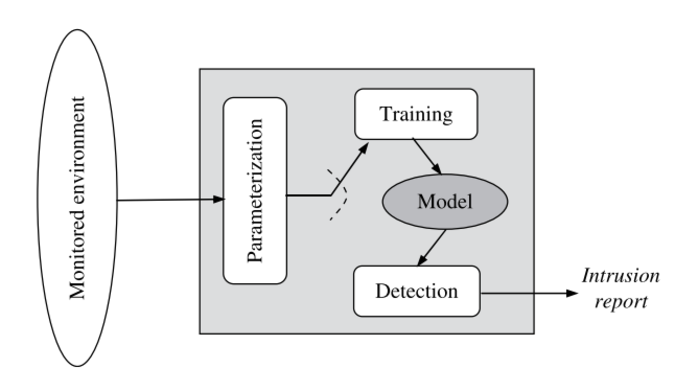
\includegraphics{thesis_files/figure-latex/unnamed-chunk-10-1} 

}

\caption{Functional Architecture of an A-NIDS}\label{fig:unnamed-chunk-10}
\end{figure}

Most IDSs found in the market-place are commonly network,
signature-based IDSs and although anomaly-based detection systems are
relatively immature, they provide a greater possibility of detecting
unknown attacks. The trade-off between the two types of systems are
primarily in the accuracy with which they detect a real attack, or an
anomaly. Properly configured signature-based systems rarely raise false
alarms, but unlike anomaly-based systems, are less capable of detecting
novel attacks.

Until relatively recently, the application of IDSs to SCADA systems was
not prevalent, however there has been increasing interest and different
approaches and implementations can be seen in the
literature.{[}20--24{]}

\newpage

\section{Techniques of Network Intrusion
Detection}\label{techniques-of-network-intrusion-detection}

Numerous anomaly-based methods and techniques have been studied and
implemented in detecting network intrusions. These include statistical,
data mining and machine learning.{[}7, 21, 22, 25--39{]} Figure 8
provides a brief summary of these techniques.

\subsection{Statistical}\label{statistical}

Statistical approaches are based on either setting thresholds and
applying them to specific variables, or are based on changes in
distributions over a period of time observed. In the first case, an
upper and lower bound are established to define an appropriate range of
values for the individual variables measured. Earlier methods began by
using the univariate model where single variables are analyzed, and
later, multivariate models were applied in which highly correlated
metrics were used, as they were considered to be more effective at
distinguishing anomalies. In the second case, considered as a
time-series model, a window of data is used to compute the mean of its
distribution in order to determine the thresholds.{[}22, 41--45{]}

\subsection{Data Mining}\label{data-mining}

Data mining, also known as Knowledge Discovery in Databases (KDD), is
the the process of extracting information and detecting interesting
patterns from data. A good deal of work is involved prior to the mining
process in understanding and preparing the data for the mining process
and analysis. Some data mining techniques include, but are not limited
to association rules, language processing, and decision trees and
consist of such algorithms as Apriori, K-Means, and K-Medoids to mention
a few.{[}46--60{]}

\subsection{Machine Learning}\label{machine-learning}

In the machine learning approach an algorithm is trained to learn
against a set of data that has been previously identified, or labeled,
and as more data becomes available, the greater the accuracy of the
model. Prominent methods of machine learning are Bayesian and Neural
Networks, SVM, kNN, clustering and outlier detection.{[}44, 61--68{]}

Similarities and overlap can be seen between the techniques above as
they have evolved and originated from, and are intersections of, the
fields of computer science, statistics, artificial intelligence, and
database systems. Each of these methods presents its advantages and
drawbacks, and in evaluating them, it will be important to consider the
time and complexity in the processing and analysis of data, the
availability of previously identified data, as well as the legibility of
results, that is, how easily the results can be read and interpreted.

\begin{figure}

{\centering 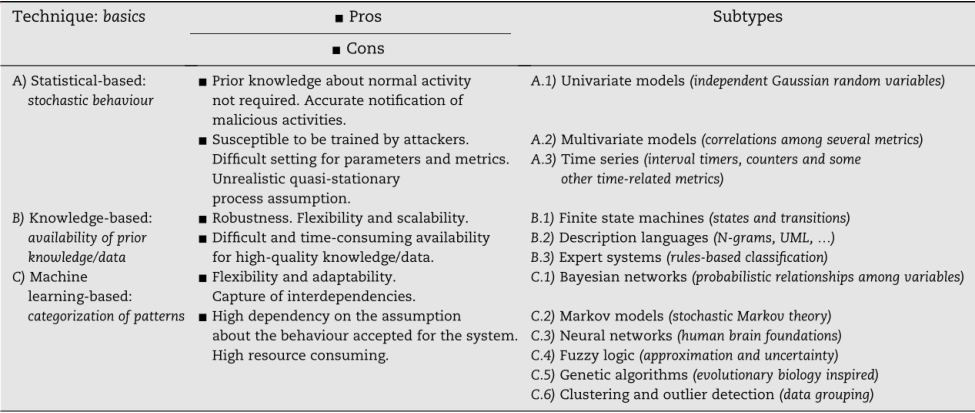
\includegraphics{thesis_files/figure-latex/unnamed-chunk-11-1} 

}

\caption{Fundamentals of A-NIDS Techniques}\label{fig:unnamed-chunk-11}
\end{figure}

\clearpage

\section{Data Source}\label{data-source}

It is usual for network data to contain private and sensitive
information, and therefore a limited number of datasets exist for
testing. Consequently, it is difficult to evaluate and assess the
accuracy and validity, as well as to make comparisons across the
different methods applied in anomaly detection.

One of the only publicly available datasets containing network traffic
data has been provided by the US Defense Advanced Research Projects
Agency (DARPA).{[}69{]} Network IDS analysis and studies have commonly
been carried out using the DARPA dataset. In this study, the analysis
has been completed using data acquired from a simulated testbed, the
Virtual Scada Box.

\subsection{HNS and Virtual Scada Box}\label{hns-and-virtual-scada-box}

diateam has developed a system, hynesim (HNS), that is a distributed
platform used in simulating complex information and network systems.
With its ergonomic graphical user interface, hynesim has a distributed
architecture and modular system, which allows for the inter-connection
between real, as well as virtual systems.

Incorporated into Virtual Scada Box, hynesim is the principal component
where there is a virtual system that simulates a water treatment plant.
Virtual Scada Box includes components such as the PLCs, HMIs, and a
virtual water pump that have been connected over a TCP/IP network.

The data analyzed were derived from a simulated network running on the
Virtual Scada Box. A packet capture file was created via Wireshark,
which captured the network traffic simulated over a virtual SCADA
network.

\subsection[PCAP]{PCAP\footnote{\url{https://www.winpcap.org/ntar/draft/PCAP-DumpFileFormat.html}}}\label{pcap2}

This section describes the format used for the packet capture file
format of the dumped packets.

The general structure is in a block format as shown below, with the
following fields:

\begin{itemize}
\itemsep1pt\parskip0pt\parsep0pt
\item
  Block Type (32 bits) - unique value that identifies the block.
\item
  Block Total Length - total size in bytes.
\item
  Block Body - content.
\item
  Block Total Length - total size in bytes. that is duplicated for
  allowing backward file navigation.
\end{itemize}

\newpage

\begin{verbatim}

0                   1                   2                   3
0 1 2 3 4 5 6 7 8 9 0 1 2 3 4 5 6 7 8 9 0 1 2 3 4 5 6 7 8 9 0 1
+-+-+-+-+-+-+-+-+-+-+-+-+-+-+-+-+-+-+-+-+-+-+-+-+-+-+-+-+-+-+-+-+
|                          Block Type                           |
+-+-+-+-+-+-+-+-+-+-+-+-+-+-+-+-+-+-+-+-+-+-+-+-+-+-+-+-+-+-+-+-+
|                      Block Total Length                       |
+-+-+-+-+-+-+-+-+-+-+-+-+-+-+-+-+-+-+-+-+-+-+-+-+-+-+-+-+-+-+-+-+
/                          Block Body                           /
/          /* variable length, aligned to 32 bits */            /
+-+-+-+-+-+-+-+-+-+-+-+-+-+-+-+-+-+-+-+-+-+-+-+-+-+-+-+-+-+-+-+-+
|                      Block Total Length                       |
+-+-+-+-+-+-+-+-+-+-+-+-+-+-+-+-+-+-+-+-+-+-+-+-+-+-+-+-+-+-+-+-+    
    
\end{verbatim}

\subsection{MODBUS/TCP Packets}\label{modbustcp-packets}

Example MODBUS packets, with MODBUS data values:

\subsubsection{Request}\label{request}

\begin{verbatim}

65  572.608117000   192.168.12.51   192.168.12.253  MODBUS/TCP  66     query: trans:
20; unit:   1, func:   4: Read input registers

0000  00 80 f4 0f 35 aa 00 18  63 37 9b 5b 08 00 45 00   ....5... c7.[..E.
0010  00 34 41 35 40 00 80 06  1f 0e c0 a8 0c 33 c0 a8   .4A5@... .....3..
0020  0c fd 09 c3 01 f6 05 1a  47 65 63 b7 1f c5 50 18   ........ Gec...P.
0030  fa 14 3e 57 00 00 00 14  00 00 00 06 01 04 00 00   ..>W.... ........
0040  00 01    
    
\end{verbatim}

\subsubsection{Response}\label{response}

\begin{verbatim}

66  572.617795000   192.168.12.253  192.168.12.51   MODBUS/TCP  65  response: trans:
20; unit:   1, func:   4: Read input registers

0000  00 18 63 37 9b 5b 00 80  f4 0f 35 aa 08 00 45 00   ..c7.[.. ..5...E.
0010  00 33 89 26 40 00 40 06  17 1e c0 a8 0c fd c0 a8   .3.&@.@. ........
0020  0c 33 01 f6 09 c3 63 b7  1f c5 05 1a 47 71 50 18   .3....c. ....GqP.
0030  22 08 9f 5a 00 00 00 14  00 00 00 05 01 04 02 00   "..Z.... ........
0040  75
    
\end{verbatim}

\newpage

\section{Exploratory Data Analysis}\label{exploratory-data-analysis}

Originally championed by John Tukey{[}70{]}, Exploratory Data Analysis
(EDA) is an initial approach to understanding a data set in order to get
a ``feel'' for the data, to summarizing its essential characteristics
and to studying patterns in the data. Moreover, exploratory data
analysis frequently incorporates graphical representations beyond using
quantitative techniques.

Conducting EDA possibly gives further insight into the form and
structure of the data set, in addition to extracting value, visualizing
the data, and just as importantly, in communicating it. The initial
phase of exploratory data analysis was conducted in order to better
understand the data. This section presents a short list of statistical
terminology, followed by the exploratory data analysis carried out on
the network traffic data captured over the simulated SCADA network and
shows the different ways they can be visualized. The analysis, reporting
and visualization was done using R and RStudio.

\subsection{Statistical Definitions}\label{statistical-definitions}

\subsubsection{Mean}\label{mean}

The (arithmetic) mean is a measure of central tendency, which is a
single value which represents an average of the sample or population. It
is calculated by dividing all the observations by the number of
observations.

\subsubsection{Median}\label{median}

Another measure of central tendency is the median, however, in this
case, the median is determined by first ordering the observations by
magnitude. Then the median is taken as the value which falls in the
middle, or the average of the two middle values in the case of an even
number of observations. The median is better suited when there are
observations, or outliers, that fall way outside the norm. These are
extreme values that differ greatly from other values in the data set.

\subsubsection{Variance}\label{variance}

The variance is the expected value of the squared differences between
the random variables and its mean that is always positive. It gives an
indication of how far apart the values are from the mean and each other.

\[ var[X] = E[(X - E[X])^2] \]

\subsubsection{Standard Deviation}\label{standard-deviation}

The standard deviation is a measure of dispersion, or how spread out a
random variable is around its mean. It is calculated as the square root
of the variance and is, unlike the variance, expressed in the same terms
(unit) as the data.

\[ \sigma = \sqrt(var[X]) \]

\subsubsection{Covariance}\label{covariance}

A measure of how closely two variables change, or vary together is the
covariance. Random variables whose covariance is 0 is said to be
uncorrelated.

\[ \sigma(X, Y) = E[(X - E[X])(Y-E[Y])] \]

\subsubsection{Correlation}\label{correlation}

Correlation is the strength between the relationship of, or dependence
between, two variables whose value have been normalized and is typically
bounded between the values of -1 and 1. It describes the magnitude and
the direction of the relationship. If the correlation is positive, their
values increase together, and if it is negative, one value decreases as
the other value increases.

\[ \rho(X, Y) = \sigma(X, Y) / (\sigma [X] \sigma [Y]) \]

\subsection{Visual Representations}\label{visual-representations}

\subsubsection{Pie chart}\label{pie-chart}

A pie chart is a circular diagram representing numerical proportions as
slices of the pie.

\subsubsection{Scatter plot}\label{scatter-plot}

A diagram showing a collection of points as depicted by the coordinates
between two variables on a plane. One axis represents the independent
variable, whereas the other represents the dependent variable.

\subsubsection{Histogram}\label{histogram}

A graphical representation which shows the distribution of continuous
numerical values is a histogram and can be representative of a
probability distribution. A frequency histogram is a univariate
graphical way to show frequency counts of a value showing bars of
different heights.

\subsubsection{Bar chart}\label{bar-chart}

Similar to a histogram, a bar chart shows the distribution of values of
a given variable with the data categorized.

\subsubsection{Boxplot}\label{boxplot}

An effective and graphical method for visualizing outliers is the
boxplot. It displays the data in terms of interquartiles, where outliers
are indicated as individual points. (Figure 9: Boxplot Image
Source{[}71{]})

\begin{figure}

{\centering 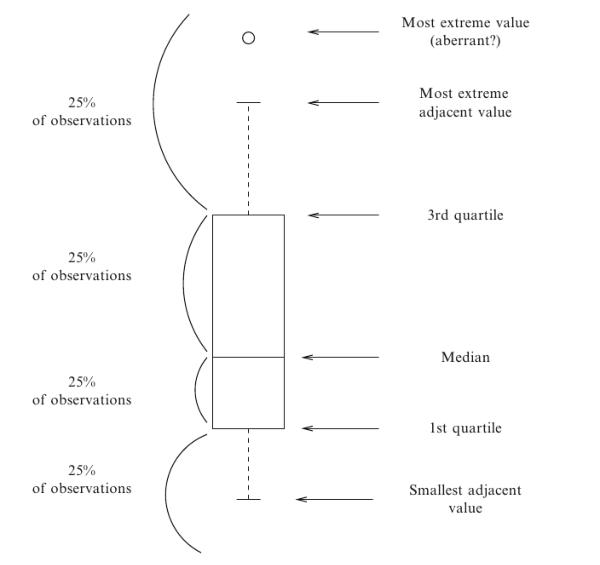
\includegraphics{thesis_files/figure-latex/unnamed-chunk-15-1} 

}

\caption{Boxplot}\label{fig:unnamed-chunk-15}
\end{figure}

\subsubsection{Heat Map}\label{heat-map}

A heat map displays data in a matrix where the values are represented by
a range of colors. Typically displayed in 2D, larger values are usually
shown in darker colors and smaller values in lighter colors on a heat
map. They can also be accompanied by a dendrogram, a tree diagram that
illustrates clusters.

\subsubsection{Network Graph}\label{network-graph}

Modeling the relations between objects, another mathematical structure
is the graph comprised of nodes, or vertices, and edges. Depending on
the nature of the relationship, a graph may be either cyclic or acyclic,
directed or undirected. Attributes of a node or edge may be reflected in
the graph as well.

\subsection{Data Analysis}\label{data-analysis}

Below is a summary of the packet capture file that was created under
``normal'' conditions over the virtual SCADA network.

\begin{longtable}[c]{@{}ll@{}}
\toprule\addlinespace
\textbf{capture\_schneider\_20150903\_normal.pcapng} &
\\\addlinespace
\midrule\endhead
\textbf{File} &
\\\addlinespace
Length: & 3969470 bytes
\\\addlinespace
Format: & Wireshark - pcapng
\\\addlinespace
Encapsulation: & Ethernet
\\\addlinespace
Packet size limit: & 65535
\\\addlinespace
\textbf{Time} &
\\\addlinespace
First packet: & 2015-09-03 15:26:26
\\\addlinespace
Last packet: & 2015-09-03 15:36:29
\\\addlinespace
Elapsed: & 00:10:02
\\\addlinespace
\textbf{Traffic Captured} &
\\\addlinespace
Packets & 39784
\\\addlinespace
B/t first and last pkt & 602,865 sec
\\\addlinespace
Avg. packets/sec & 65,992
\\\addlinespace
Avg. packet size & 65,343 bytes
\\\addlinespace
Bytes & 2599593
\\\addlinespace
Avg. bytes/sec & 4312,063
\\\addlinespace
Avg. Mit/sec & 0,034
\\\addlinespace
\bottomrule
\end{longtable}

Once the network traffic was captured and saved in a PCAP file,
Wireshark provides the capability to export the raw data into various
comma delimited files in order to do further analysis. Exported files
were created with TCP endpoints, TCP conversations, as well as the
entire pcap file, each as a CSV file. (Appendix B)

\subsection{Network Analysis}\label{network-analysis}

\subsubsection{Network Graph and
Topology}\label{network-graph-and-topology}

Figure 10 depicts the network topology of the components and end points
on the simulated network.

\begin{figure}[h]

{\centering 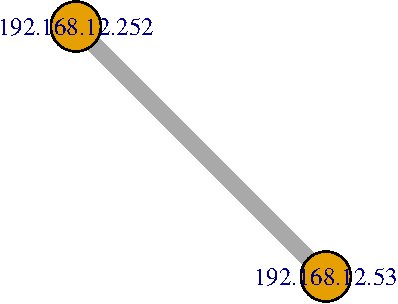
\includegraphics{thesis_files/figure-latex/warning-1} 

}

\caption{SCADA Network Graph}\label{fig:warning}
\end{figure}

The following Tables 3-7 list the data extracted from the packet capture
file:

\begin{longtable}[c]{@{}lllr@{}}
\toprule\addlinespace
ip.src & ip.dst & mbtcp.modbus.unit\_id & count
\\\addlinespace
\midrule\endhead
192.168.12.53 & 192.168.12.253 & 1 & 19323
\\\addlinespace
192.168.12.253 & 192.168.12.53 & 1 & 19323
\\\addlinespace
\bottomrule
\addlinespace
\caption{Source / Destination / UnitID}
\end{longtable}

\begin{longtable}[c]{@{}lr@{}}
\toprule\addlinespace
ip.src & count
\\\addlinespace
\midrule\endhead
192.168.12.53 & 19323
\\\addlinespace
192.168.12.253 & 19323
\\\addlinespace
\bottomrule
\addlinespace
\caption{Sources}
\end{longtable}

\begin{longtable}[c]{@{}lr@{}}
\toprule\addlinespace
ip.dst & count
\\\addlinespace
\midrule\endhead
192.168.12.253 & 19323
\\\addlinespace
192.168.12.53 & 19323
\\\addlinespace
\bottomrule
\addlinespace
\caption{Destination}
\end{longtable}

\begin{longtable}[c]{@{}lll@{}}
\toprule\addlinespace
ip.dst & mbtcp.modbus.unit\_id & ip.dst.unit\_id
\\\addlinespace
\midrule\endhead
192.168.12.253 & 1 & 192.168.12.253/1
\\\addlinespace
192.168.12.53 & 1 & 192.168.12.53/1
\\\addlinespace
\bottomrule
\addlinespace
\caption{Destination / UnitID}
\end{longtable}

\newpage

\begin{longtable}[c]{@{}lll@{}}
\toprule\addlinespace
ip.src & mbtcp.modbus.func\_code & src.func
\\\addlinespace
\midrule\endhead
192.168.12.53 & 4 & 192.168.12.53/4
\\\addlinespace
192.168.12.253 & 4 & 192.168.12.253/4
\\\addlinespace
\bottomrule
\addlinespace
\caption{Source / Function Code}
\end{longtable}

\subsection{Packet Analysis}\label{packet-analysis}

Figure 11 depicts a boxplot indicating packet size.

\begin{figure}[h]

{\centering 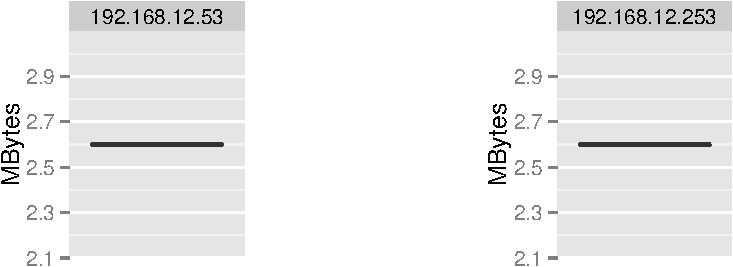
\includegraphics{thesis_files/figure-latex/unnamed-chunk-21-1} 

}

\caption{Source Packet Size Boxplot}\label{fig:unnamed-chunk-21}
\end{figure}

\subsubsection{MODBUS/TCP Request/Response Packet Statistics (Appendix
C)}\label{modbustcp-requestresponse-packet-statistics-appendix-c}

MODBUS/TCP \textbf{requests} are identified by packets having
destination port number 502 (Figure 13).

\begin{figure}[h]

{\centering 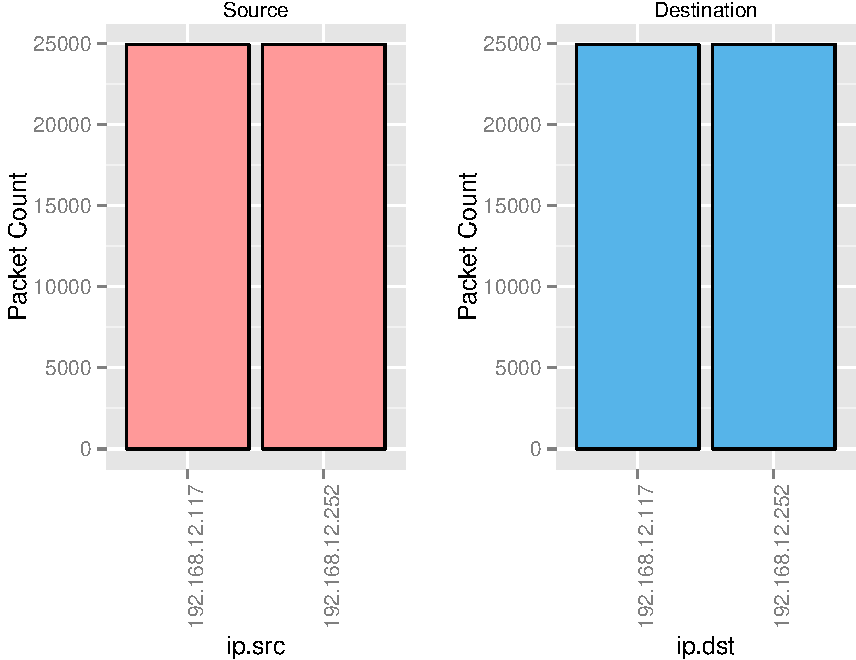
\includegraphics{thesis_files/figure-latex/unnamed-chunk-22-1} 

}

\caption{Boxplot of Request Packets}\label{fig:unnamed-chunk-22}
\end{figure}

MODBUS/TCP \textbf{responses} are identified by packets having source
port number 502 (Figure 14).

\begin{figure}[h]

{\centering 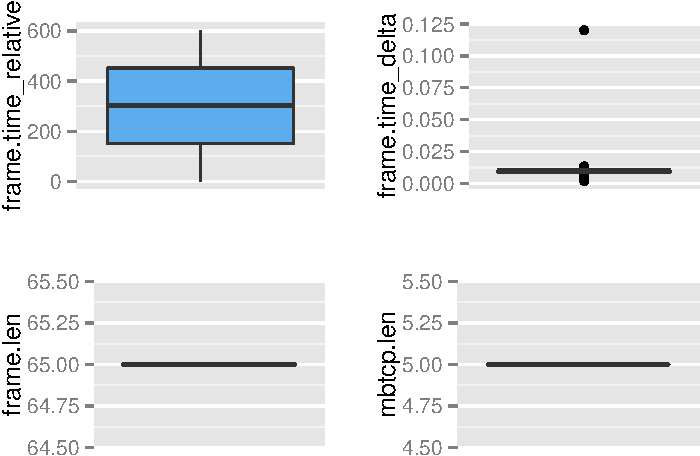
\includegraphics{thesis_files/figure-latex/unnamed-chunk-23-1} 

}

\caption{Boxplot of Response Packets}\label{fig:unnamed-chunk-23}
\end{figure}

\clearpage

\begin{figure}[h]

{\centering 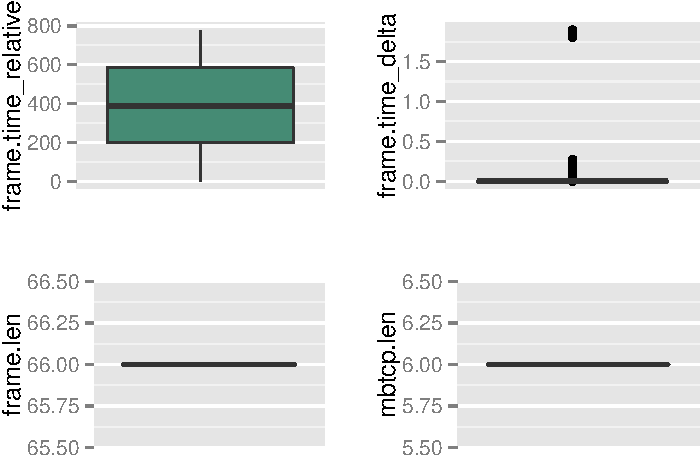
\includegraphics{thesis_files/figure-latex/unnamed-chunk-24-1} 

}

\caption{Bar Charts of Packet Counts}\label{fig:unnamed-chunk-24}
\end{figure}

\begin{figure}[h]

{\centering 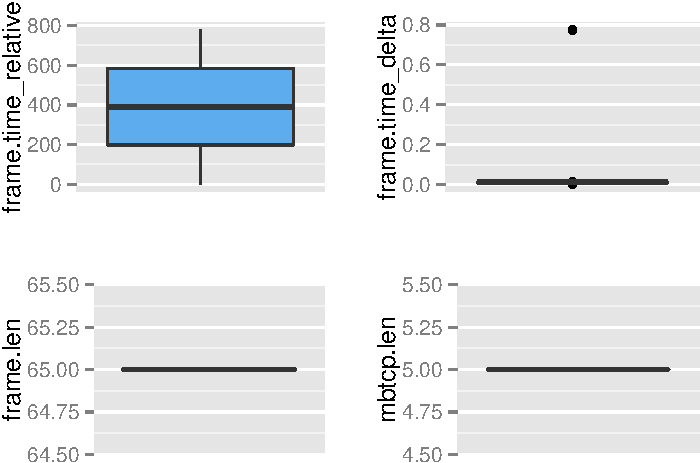
\includegraphics{thesis_files/figure-latex/unnamed-chunk-26-1} 

}

\caption{Scatterplot of Time as a Function of Frame Number}\label{fig:unnamed-chunk-26}
\end{figure}

\begin{figure}[h]

{\centering 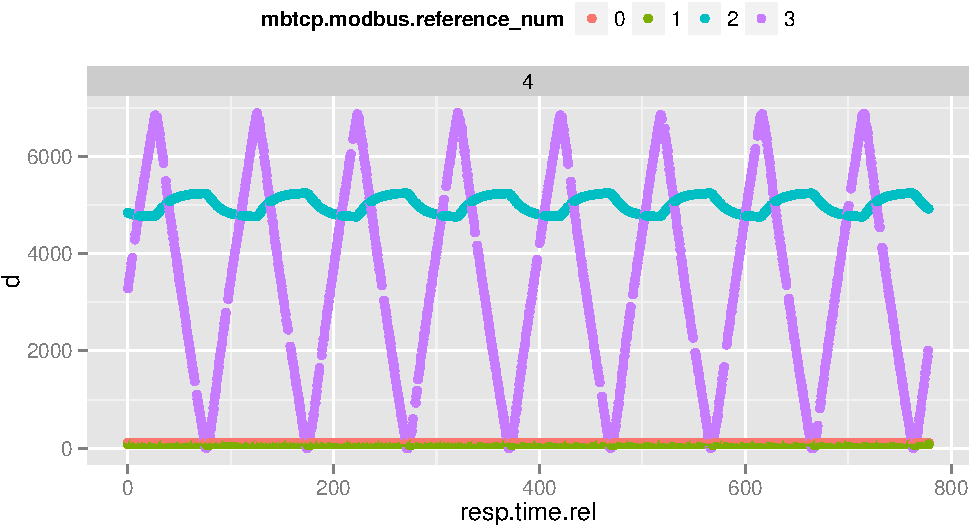
\includegraphics{thesis_files/figure-latex/unnamed-chunk-27-1} 

}

\caption{Boxplot of Modbus/TCP Data Length}\label{fig:unnamed-chunk-27}
\end{figure}

\begin{figure}[h]

{\centering 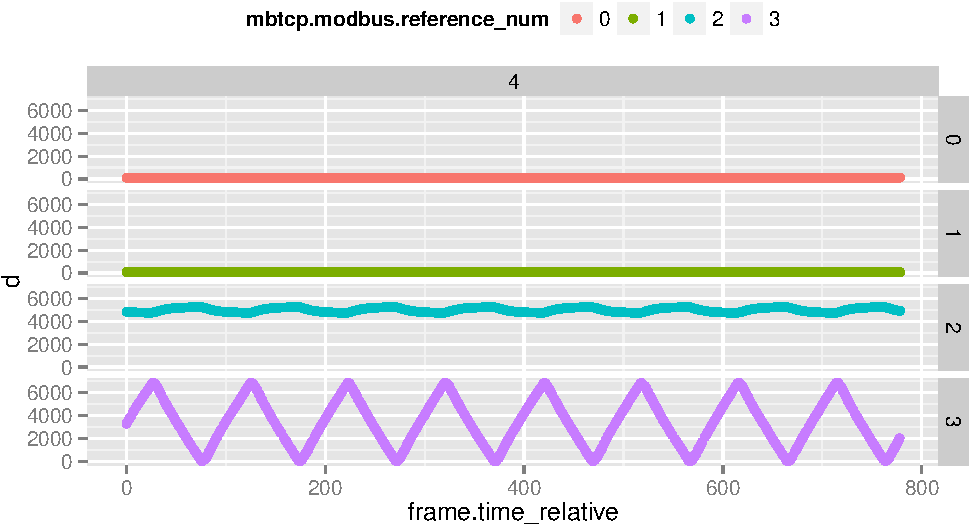
\includegraphics{thesis_files/figure-latex/unnamed-chunk-28-1} 

}

\caption{Graph of MODBUS Data Values over Time by MODBUS  Reference Number}\label{fig:unnamed-chunk-28}
\end{figure}

\begin{figure}[h]

{\centering 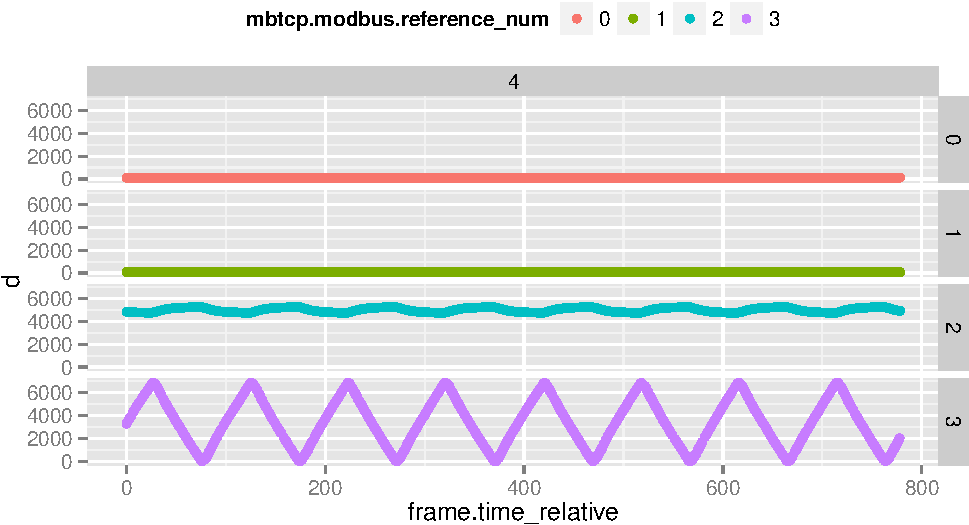
\includegraphics{thesis_files/figure-latex/unnamed-chunk-29-1} 

}

\caption{Graph of MODBUS Data Values over Time by Function Code}\label{fig:unnamed-chunk-29}
\end{figure}

\subsubsection[MODBUS/TCP Data Analysis]{MODBUS/TCP Data\footnote{\url{https://www.wireshark.org/docs/dfref/m/mbtcp.html}}
Analysis}\label{modbustcp-data3-analysis}

The following analysis was done over the previous dataset that was
processed to merge response packet to the request packet of the same
transaction. An additional field ``d'' is the data field ``resp.data''
converted from a hex to a decimal value. (Appendix D)

\subsubsection{MODBUS Data Value
Statistics}\label{modbus-data-value-statistics}

\begin{verbatim}
   resp.func.code mbtcp.modbus.reference_num count d.min     d.mean d.max
1:              4                          0 10273   112  112.00000   112
2:              4                          1 11737    64   81.31448    84
3:              4                          2  1468  4758 5005.32493  5242
4:              4                          3  1467     0 3392.64554  6890
          d.sd min.resp.time.rel min.resp.time.rel
1:    0.000000          0.196988          778.1052
2:    3.891773          0.246152          778.1175
3:  179.359760          0.185127          778.0571
4: 2074.517793          0.270168          777.6427
\end{verbatim}

\clearpage

Under normal activity, it is typical to see MODBUS function code 4
(0x04) requested, as shown in all figures grouped by function code. This
is the function code that corresponds to Read Input Registers.

It can also be seen in Figures 17, 18 and 22 how cyclical the processes
are in the system.

\begin{figure}[h]

{\centering 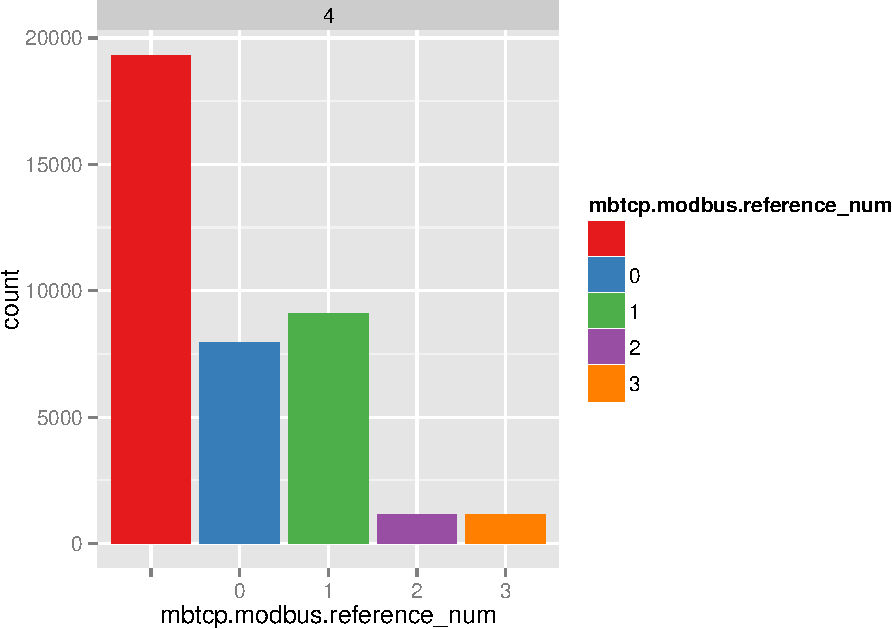
\includegraphics{thesis_files/figure-latex/unnamed-chunk-31-1} 

}

\caption{Bar Chart of MODBUS Reference Numbers by Function Code}\label{fig:unnamed-chunk-31}
\end{figure}

In Figures 17-20, reference numbers refer to the register number of the
PLC devices. The reference numbers indicate the following:

\begin{itemize}
\itemsep1pt\parskip0pt\parsep0pt
\item
  0 - state
\item
  1 - errors
\item
  2 - water level
\item
  3 - pump speed
\end{itemize}

\begin{figure}[h]

{\centering 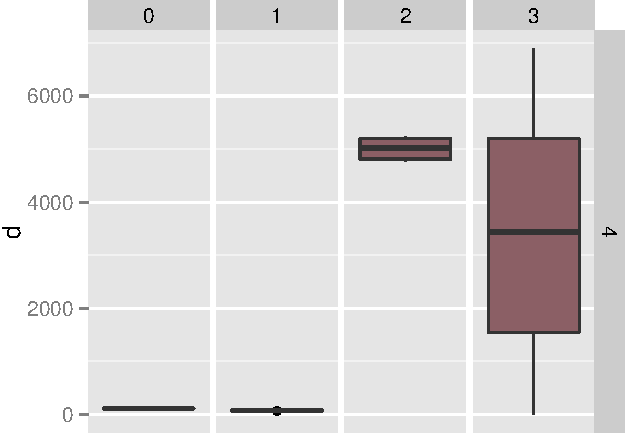
\includegraphics{thesis_files/figure-latex/unnamed-chunk-32-1} 

}

\caption{Boxplot of MODBUS Data Values by Function and Reference Number}\label{fig:unnamed-chunk-32}
\end{figure}

\begin{figure}[h]

{\centering 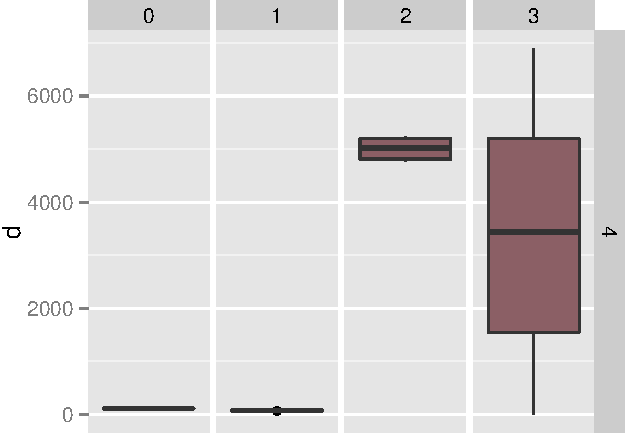
\includegraphics{thesis_files/figure-latex/unnamed-chunk-33-1} 

}

\caption{Scatterplot Matrix of Pairs of Variables}\label{fig:unnamed-chunk-33}
\end{figure}

\clearpage

\begin{figure}[h]

{\centering 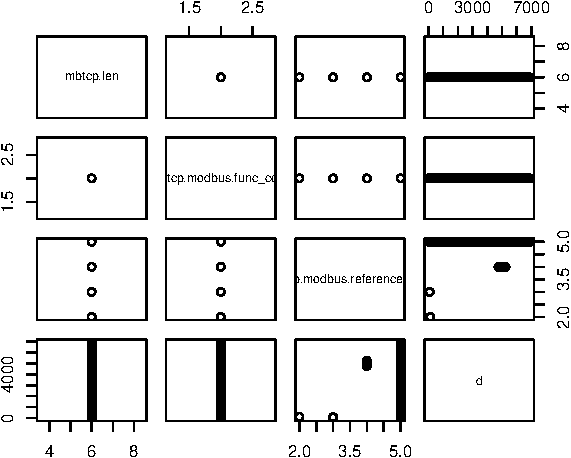
\includegraphics{thesis_files/figure-latex/unnamed-chunk-34-1} 

}

\caption{3D Scatterplot of MODBUS Reference Number
 and Data Over Time for Function Code 4}\label{fig:unnamed-chunk-34}
\end{figure}

\clearpage

\section{Proof of Concept}\label{proof-of-concept}

The SCAD@COPS proof of concept incorporates the methods as outlined in
{[}3, 4{]}, which define the architectural and signature-based detection
system, and the last component being the anomaly-based detection system.
The signature-based IDS component was previously implemented and
configured using Suricata. The initial POC will contain an anomaly-based
IDS using statistical methods, which is what this project has
concentrated on.

\subsection{Architecture Overview}\label{architecture-overview}

Network IDSs are utilized for security monitoring, but are themselves
also vulnerable and exposed to attacks. {[}3{]} proposes an architecture
for the IDS sensor devices and software to minimize the possibility of
attacks on it. The two approaches presented are to:

\begin{itemize}
\itemsep1pt\parskip0pt\parsep0pt
\item
  reinforce software security- reduce the area of attack, remove unused
  applications and services, and reduce permissions and privileges of
  important processes
\item
  isolate system components- partition and separation between users and
  processes via virtualization
\end{itemize}

In Figure 23, an example is shown of the placement of the IDS and its
supporting DB, connected to other SCADA components.

\begin{figure}[h]

{\centering 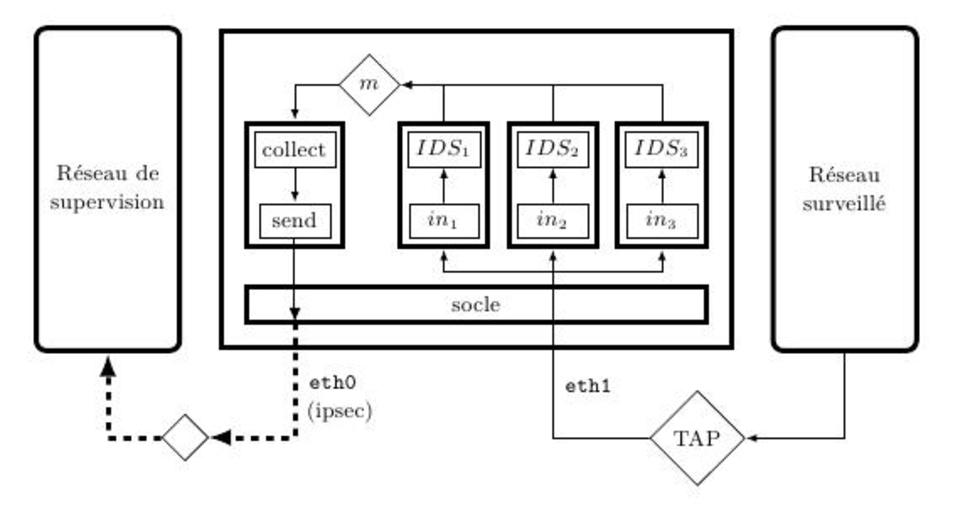
\includegraphics{thesis_files/figure-latex/unnamed-chunk-35-1} 

}

\caption{Technical Architecture}\label{fig:unnamed-chunk-35}
\end{figure}

Based on the recommendations of {[}3{]}, in order to address the
security concerns of the IDS appliance itself, the architecture contains
a partition of the various components and isolates each IDS instance
from one another, as can be seen in Figure 24. All resources are set to
read-only mode, with limited authorized access. For maintenance, updates
are deposited in a dedicated area and then copied over to another
reserved area that are either executed by a scheduled job or via a
trigger. A Mirabox is used as the embedded system running the latest
stable version of Debian and virtual private networks to communicate
between the internal IDS and the supervisory system (Figure 24).{[}3{]}

{[}4{]} advises the strategic placement of the monitoring devices
throughout the SCADA system on a dedicated network for supervision, and
presents the two different approaches of a centralized or a distributed
system.

\begin{figure}[h]

{\centering 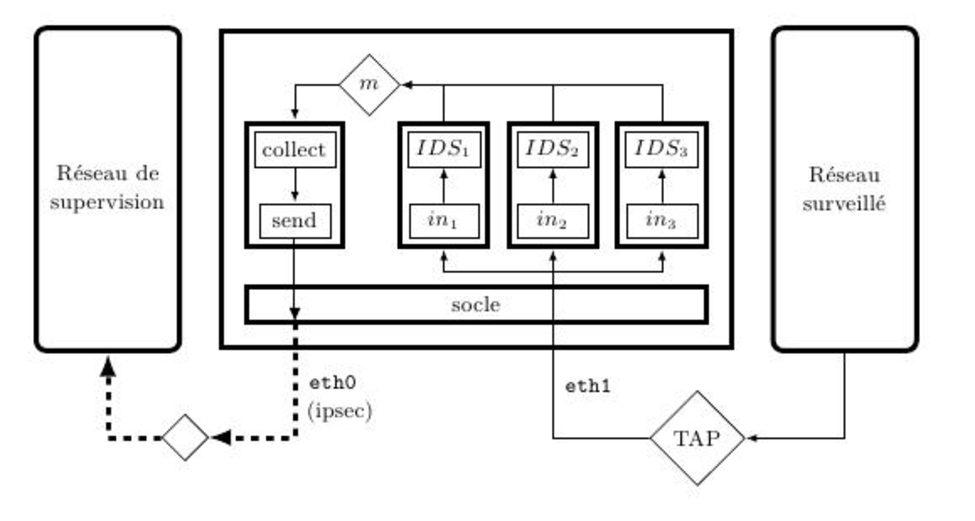
\includegraphics{thesis_files/figure-latex/unnamed-chunk-36-1} 

}

\caption{Architecture of secure IDS }\label{fig:unnamed-chunk-36}
\end{figure}

\subsubsection{Signature-based IDS}\label{signature-based-ids}

In {[}3{]} and {[}4{]}, the signature based IDS is described and the use
of the Suricata IDS software with MODBUS protocol are proposed. Rules
are configured that conform to, and verify the correct and normal
behaviour of a SCADA system.

\subsubsection{Anomaly-based IDS}\label{anomaly-based-ids}

In the scope of the SCAD@COPS project, the anomaly-based component will
be derived from various statistical properties, that will be discussed
subsequently in Chapter 10.

\subsection{Implementation}\label{implementation}

All software and tools applied and implemented in the SCAD@COPS project
are free and open source (Appendix E).

\subsubsection{Process Flow}\label{process-flow}

Figure 25 shows the steps involved in the entire process from acquiring
the data, computation and analysis, to setting the IDS to detection
mode.

\begin{itemize}
\itemsep1pt\parskip0pt\parsep0pt
\item
  Step 1: Data Acquisition During Normal Activity - From the IDS
  appliance, sniff the network traffic, extract and store data in a
  database.
\item
  Step 2: Statistical Process and Analysis

  \begin{itemize}
  \itemsep1pt\parskip0pt\parsep0pt
  \item
    2.1 Process data - Perform any transformation, filtering and data
    cleansing necessary.
  \item
    2.2 Calculate and determine statistical measures.
  \item
    2.3 Configure appliance with statistical parameters.
  \end{itemize}
\item
  Step 3: Detection Mode - Appliance is set to detection mode.
\end{itemize}

\begin{figure}[h]

{\centering 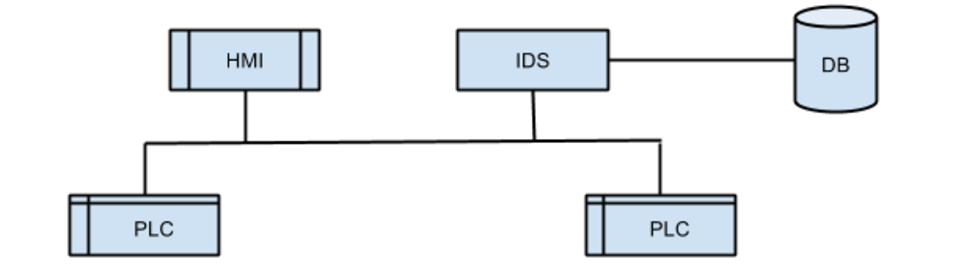
\includegraphics{thesis_files/figure-latex/unnamed-chunk-37-1} 

}

\caption{Process Flow}\label{fig:unnamed-chunk-37}
\end{figure}

\subsubsection{Data Acquisition}\label{data-acquisition}

As illustrated in Section 9.1, Figure 24, the data is acquired by one of
the components of the NIDS, which has been configured to only monitor
network traffic:

\begin{itemize}
\itemsep1pt\parskip0pt\parsep0pt
\item
  Wireshark - An initial packet capture file was created over the
  simulated network traffic using Wireshark. Using its export
  facilities, various files were created for further analysis, with
  information such as TCP endpoints, conversations, etc.
\item
  TShark - The pertinent variables pertaining to the MODBUS/TCP
  application protocol enclosed in the packet data were extracted and
  parsed by TShark.
\end{itemize}

\subsubsection{Statistical Analysis and
Processing}\label{statistical-analysis-and-processing}

The statistical process was implemented using various components to
handle specific steps. Each component used was initially selected to
manage a particular task of the process according to its ease and
efficiency of development, as well as its processing time (Appendix F).
Once captured from the monitoring device on the IDS appliance, the
packet capture file can be processed offline. Configuration files are
subsequently generated in JSON format after the statistical
computations, which can then be uploaded to the IDS appliance.

\begin{figure}[h]

{\centering 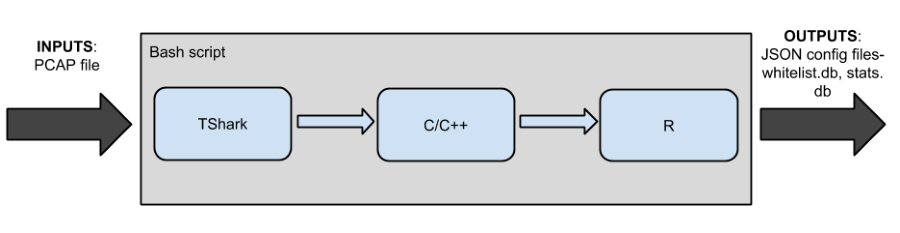
\includegraphics{thesis_files/figure-latex/unnamed-chunk-38-1} 

}

\caption{Statistical Computational Process}\label{fig:unnamed-chunk-38}
\end{figure}

\newpage

The components are as follows, and depicted in Figure 26:

\begin{itemize}
\itemsep1pt\parskip0pt\parsep0pt
\item
  bash/Unix - The entire procedure is handled by a bash shell script,
  executing other scripts or programs.
\item
  C/C++ - Initial analysis was completed in R, however, for greater
  efficiency, some data preprocessing, including merging and
  transformations were programmed in C/C++.
\item
  R - Most statistical computations and configuration file generations
  were done using many R libraries and programmed in R scripts.
\end{itemize}

\clearpage

\section{Statistical Measures and
Features}\label{statistical-measures-and-features}

Regardless of the predictive method or technique chosen, the predictive
accuracy and performance of any model is influenced by the features
selected, and is therefore important to take into consideration. Feature
selection is the reduction of the input variables. Whether it be in the
field of statistics, data mining, or machine learning, massive amounts
of data that are handled can greatly benefit from the careful selection
of relevant features. In addition, removing redundancies also improves
the efficiency and having both allows for further increased accuracy and
reduction in complexity. However, there should be an appropriate
selection of features so as to prevent any loss of information.{[}72,
73{]}

Depending on the size of the dataset and the number of features, or
variables, the selection process may simply be done by a domain expert
who has been trained in a particular field and has the expertise to
determine which features are deemed as important. Although this may be
sufficient in some cases, enormous amounts of data and variables make
the process more complex, and less effective and efficient. More
sophisticated methods go through a learning process in order to detect
patterns with less human intervention.

An example of applying feature selection is in the area of text mining
where unstructured data can be comprised of millions of words. Using
such techniques as stop word elimination and stemming, the
dimensionality is notably reduced. Principal component analysis is
another statistical procedure by which the data can be transformed and
represented as its eigenvalues and eigenvectors.

Network based intrusion detection has been studied for some time and can
be implemented by using conventional network variables.{[}43, 74{]} In
{[}36, 67{]}, the challenges of feature selection in the context of
anomaly detection in industrial systems are discussed.

The first version of the SCAD@COPS network intrusion detection device
for industrial systems will be based on simple statistical variables
that have been chosen by an expert in the domain of cyber security with
experience in SCADA systems. Example configuration files generated from
the statistical process as outlined in Section 9.2.2 (Appendix G) have
been used as the parameters in the proof of concept.

\clearpage

\section{Testing and Evaluation}\label{testing-and-evaluation}

Security agents supervise SCADA systems that have numerous controls and
systems to oversee, therefore the great amount of data that is presented
by the HMIs and monitoring systems can become overwhelming. In this
regard, it is important to have pertinent data and information alerted
to the security agent. An effective NIDS should be able to monitor
traffic and detect with a minimum amount of error any deviant behaviour
or characteristics that occur out of the ordinary. Such events may be
malicious as those seen in Chapter 4, as well as routine, or
spontaneous, maintenance activities.

As discussed in Section 9.2.1, the process flow depicts the phases of
the processes involved, from data acquisition, to data processing and
statistical analysis, and finally to placing the device in
``operational'' mode where network traffic may be exposed to attacks.
During the testing phase, another simulation was done with attacks
injected via Metasploit.

The test simulation exposed the routine activity running on the Virtual
Scada Box to a remote MODBUS STOP attack. Metasploit provides a means
for the attacker to end a PLC process control by sending MODBUS frames
with function code 90 (0x5a). This is used to perform administrative
commands without authentication thereby modifying the state of the PLC
between STOP and RUN. Multiple frames are sent to the PLC in order to
set it to INIT mode, and the following frames are sent to request a STOP
(Appendix H):

\begin{verbatim}
5a 01 41 ff 00
00 5a 01 04
\end{verbatim}

The packet capture file was also processed in a similar manner as the
initial PCAP file, and then a comparison was made to find differences
and anomalies between the two data sets.

The following tables list anomalies and differences detected in the
attack simulation:

\begin{longtable}[c]{@{}l@{}}
\toprule\addlinespace
ip.src
\\\addlinespace
\midrule\endhead
192.168.12.34
\\\addlinespace
\bottomrule
\addlinespace
\caption{Anomalous Sources}
\end{longtable}

\begin{longtable}[c]{@{}l@{}}
\toprule\addlinespace
ip.dst
\\\addlinespace
\midrule\endhead
192.168.12.34
\\\addlinespace
\bottomrule
\addlinespace
\caption{Anomalous Destinations}
\end{longtable}

\begin{longtable}[c]{@{}lll@{}}
\toprule\addlinespace
IP\_DST\_MODBUS\_UNIT\_ID & ip.dst & mbtcp.modbus.unit\_id
\\\addlinespace
\midrule\endhead
192.168.12.253/ & 192.168.12.253 &
\\\addlinespace
192.168.12.253/0 & 192.168.12.253 & 0
\\\addlinespace
192.168.12.34/ & 192.168.12.34 &
\\\addlinespace
192.168.12.34/0 & 192.168.12.34 & 0
\\\addlinespace
\bottomrule
\addlinespace
\caption{Anomalous Source / MODBUS Unit Pairs}
\end{longtable}

\begin{longtable}[c]{@{}lll@{}}
\toprule\addlinespace
IP\_SRC\_MAC\_ADDR & ip.src & eth.src
\\\addlinespace
\midrule\endhead
192.168.12.34/08:00:27:4a:25:6c & 192.168.12.34 & 08:00:27:4a:25:6c
\\\addlinespace
\bottomrule
\addlinespace
\caption{Anomalous Source / MAC Address Pairs}
\end{longtable}

In Table 12, we see MODBUS function code 90, which is ordinarily sent to
perform administrative commands without authentication.

\begin{longtable}[c]{@{}lll@{}}
\toprule\addlinespace
IP\_SRC\_MOD\_FUNC & ip.src & mbtcp.modbus.func\_code
\\\addlinespace
\midrule\endhead
192.168.12.253/ & 192.168.12.253 &
\\\addlinespace
192.168.12.253/90 & 192.168.12.253 & 90
\\\addlinespace
192.168.12.34/ & 192.168.12.34 &
\\\addlinespace
192.168.12.34/90 & 192.168.12.34 & 90
\\\addlinespace
192.168.12.53/ & 192.168.12.53 &
\\\addlinespace
\bottomrule
\addlinespace
\caption{Anomalous Source / MODBUS Function Code Pairs}
\end{longtable}

The difference in average frequency shown in Table 13 and 15 are
indicated by a prefix `n' for normal and `a' for attack.

\begin{longtable}[c]{@{}lll@{}}
\toprule\addlinespace
ip.src & ip.dst & mbtcp.modbus.func\_code
\\\addlinespace
\midrule\endhead
192.168.12.253 & 192.168.12.53 & 4
\\\addlinespace
192.168.12.53 & 192.168.12.253 & 4
\\\addlinespace
\bottomrule
\addlinespace
\caption{Differences in Frequency of Source/Function Code}
\end{longtable}

\begin{longtable}[c]{@{}rrr@{}}
\toprule\addlinespace
avgFrequencySec.n & avgFrequencySec.a & avgFrequencySec.diff
\\\addlinespace
\midrule\endhead
33.14408 & 33.08108 & 0.0630013
\\\addlinespace
33.14408 & 33.08108 & 0.0630013
\\\addlinespace
\bottomrule
\addlinespace
\caption{Differences in Frequency of Source/Function Code/Reference
Number}
\end{longtable}

\begin{longtable}[c]{@{}llll@{}}
\toprule\addlinespace
ip.src & ip.dst & mbtcp.modbus.func\_code & mbtcp.modbus.reference\_num
\\\addlinespace
\midrule\endhead
192.168.12.53 & 192.168.12.253 & 4 & 0
\\\addlinespace
192.168.12.53 & 192.168.12.253 & 4 & 1
\\\addlinespace
192.168.12.53 & 192.168.12.253 & 4 & 2
\\\addlinespace
192.168.12.53 & 192.168.12.253 & 4 & 3
\\\addlinespace
\bottomrule
\end{longtable}

\begin{longtable}[c]{@{}rrr@{}}
\toprule\addlinespace
avgFrequncySec.n & avgFrequncySec.a & avgFrequencySec.diff
\\\addlinespace
\midrule\endhead
13.675258 & 13.714286 & -0.0390280
\\\addlinespace
15.618557 & 15.567568 & 0.0509891
\\\addlinespace
1.962069 & 1.959184 & 0.0028853
\\\addlinespace
1.962004 & 1.959184 & 0.0028198
\\\addlinespace
\bottomrule
\end{longtable}

\clearpage

\section{Conclusion and Future Work}\label{conclusion-and-future-work}

The goal of this project was to provide the study, analysis and
conception of a proof of concept for a hybrid NIDS, focusing on the
anomaly based detection component. The work realized during this project
began with a study of the domain and the state of the art of network
intrusion detection systems in industrial control systems, SCADA systems
in particular. SCADA systems have typically been isolated and less prone
to cyber threats, but as they continue to increasingly use traditional
IT infrastructure in order to minimize costs and increase efficiency and
functionality, they become more and more vulnerable to cyber attacks. A
quality of ICSs is that their topology tends to remain static, their
protocols simple, and the traffic fairly regular.

Following the overviews of the SCADA systems and networking principles,
the MODBUS protocol and intrusion detection systems were presented, as
well as a few common attacks on SCADA systems were discussed. IDSs are
implemented as either host- or network-based and they offer a solution
to provide supervision and monitoring of SCADA systems in order to alert
to suspicious or anomalous activity. Most commercial IDSs offered are
usually signature-based, which are only able to detect previously
identified threats and defined rules of behavior. Then, different
techniques of anomaly based network intrusion detection were described.
With a growing need for robust and flexible detection of new threats as
the number of attacks increase, there is more research and advancements
in anomaly detection applying methods such as statistical, data mining
and machine learning techniques to find intelligent ways of anomaly
detection.

SCAD@COPS is a proof of concept presented by diateam, which is a hybrid
IDS that incorporates both a signature-based, as well as an
anomaly-based IDS. After having completed a comprehensive study of
intrusion detection systems and its application in SCADA systems, the
first step carried out in the development of the POC was the exploratory
data analysis of the ``normal'' network traffic data simulated by the
Virtual Scada Box. In addition to the traditional methods of using
descriptive statistics to explain the data, the various graphical and
visual manners of representing the data were exhibited. An initial
implementation of the data acquisition, data processing and statistical
computation were then executed using various tools. The project was
concluded by running another simulation in ``attack'' mode and running a
comparison against the normal data in order to detect the anomalies.

Although the first implementation of the SCAD@COPS NIDS prototype uses
rather simple statistical analysis and methods, additional research and
work can be conducted to devise further viable and effective methods for
anomaly detection. Other areas of study include more sophisticated and
advanced detection of anomalous behaviour applying machine learning, or
data mining techniques such as Neural and Bayesian networks.
Additionally, another potential area of study is Time-Series analysis.
As these methods are fairly new to the field, more work can be explored
and these methods can be exploited to further improve the accuracy and
detection of network intrusion in future versions of SCAD@COPS.

\clearpage

\section*{Appendix A}\label{appendix-a}
\addcontentsline{toc}{section}{Appendix A}

\subsection[MODBUS Function Codes]{MODBUS Function Codes\footnote{\url{https://en.wikipedia.org/wiki/Modbus}}}\label{modbus-function-codes4}

\begin{center}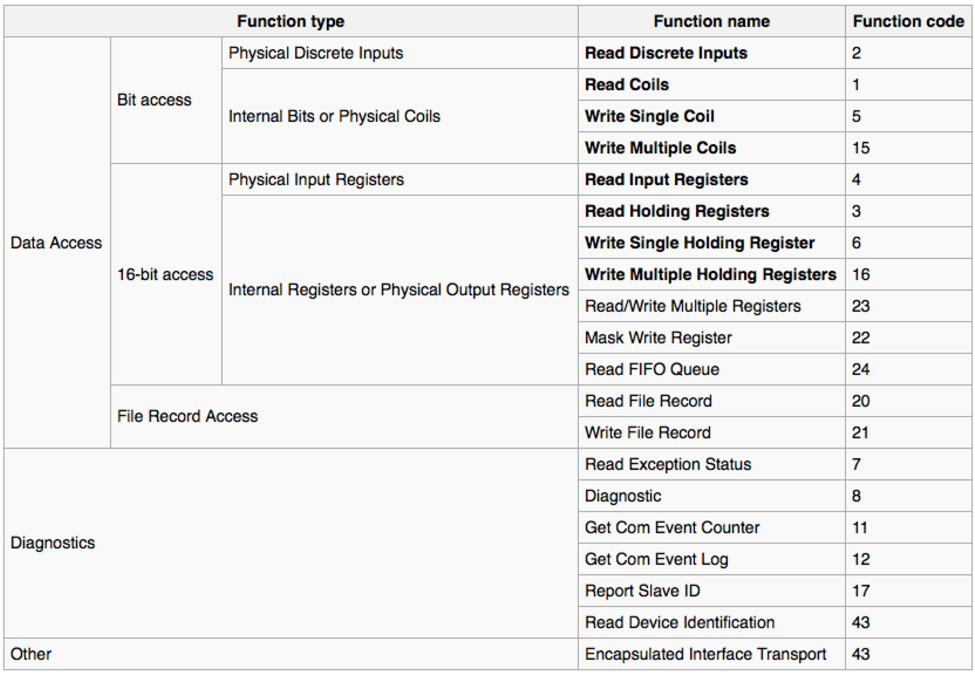
\includegraphics{thesis_files/figure-latex/unnamed-chunk-42-1} \end{center}

\clearpage

\section*{Appendix B}\label{appendix-b}
\addcontentsline{toc}{section}{Appendix B}

\subsection*{Wireshark Exports}\label{wireshark-exports}
\addcontentsline{toc}{subsection}{Wireshark Exports}

Using the export facility in Wireshark, the following are a description
of the exported files:

Entire pcap file exported in CSV format:

\begin{longtable}[c]{@{}l@{}}
\toprule\addlinespace
SCADA\_20150429\_042915.csv
\\\addlinespace
\midrule\endhead
Time
\\\addlinespace
Source
\\\addlinespace
Destination
\\\addlinespace
Protocol
\\\addlinespace
Length
\\\addlinespace
Info
\\\addlinespace
\bottomrule
\end{longtable}

List of endpoints, the traffic to and from an IP address:

\begin{longtable}[c]{@{}l@{}}
\toprule\addlinespace
SCADA\_Security\_042915\_TCP\_Endpoints.csv
\\\addlinespace
\midrule\endhead
Address
\\\addlinespace
Port
\\\addlinespace
Packets
\\\addlinespace
Bytes
\\\addlinespace
Tx.Packets
\\\addlinespace
Tx.Bytes
\\\addlinespace
Rx.Packets
\\\addlinespace
Rx.Bytes
\\\addlinespace
Latitude
\\\addlinespace
Longitude
\\\addlinespace
\bottomrule
\end{longtable}

List of conversations, the traffic between two endpoints :

\begin{longtable}[c]{@{}l@{}}
\toprule\addlinespace
SCADA\_Security\_042915\_TCP\_Conversations.csv
\\\addlinespace
\midrule\endhead
Address.A
\\\addlinespace
Port.A
\\\addlinespace
Address.B
\\\addlinespace
Port.B
\\\addlinespace
Packets
\\\addlinespace
Bytes
\\\addlinespace
Packets.A.B
\\\addlinespace
Bytes.A.B
\\\addlinespace
Packets.A.B.1
\\\addlinespace
Bytes.A.B.1
\\\addlinespace
Rel.Start
\\\addlinespace
Duration
\\\addlinespace
bps.A.B
\\\addlinespace
bps.A.B.1
\\\addlinespace
\bottomrule
\end{longtable}

\clearpage

\section*{Appendix C}\label{appendix-c}
\addcontentsline{toc}{section}{Appendix C}

\subsection*{MODBUS/TCP Request/Response Packet
Statistics}\label{modbustcp-requestresponse-packet-statistics}
\addcontentsline{toc}{subsection}{MODBUS/TCP Request/Response Packet
Statistics}

\begin{longtable}[c]{@{}lcllcll@{}}
\toprule\addlinespace
& frame.number & frame.time\_relative & frame.time\_delta & frame.len &
ip.proto & ip.version
\\\addlinespace
\midrule\endhead
& Min. : 2 & Min. : 0.1604 & Min. :0.000164 & Min. :66 & 6:19323 &
4:19323
\\\addlinespace
& 1st Qu.: 9947 & 1st Qu.:150.7170 & 1st Qu.:0.000300 & 1st Qu.:66 & NA
& NA
\\\addlinespace
& Median :19892 & Median :301.2814 & Median :0.000347 & Median :66 & NA
& NA
\\\addlinespace
& Mean :19892 & Mean :300.9954 & Mean :0.012626 & Mean :66 & NA & NA
\\\addlinespace
& 3rd Qu.:29837 & 3rd Qu.:451.8589 & 3rd Qu.:0.000368 & 3rd Qu.:66 & NA
& NA
\\\addlinespace
& Max. :39784 & Max. :602.8653 & Max. :1.905327 & Max. :66 & NA & NA
\\\addlinespace
\bottomrule
\addlinespace
\caption{Requests Summary}
\end{longtable}

\begin{longtable}[c]{@{}lcccc@{}}
\toprule\addlinespace
& ip.src & eth.src & ip.dst & eth.dst
\\\addlinespace
\midrule\endhead
& 192.168.12.253: 0 & 00:80:f4:0f:35:aa: 0 & 192.168.12.253:19323 &
00:80:f4:0f:35:aa:19323
\\\addlinespace
& 192.168.12.53 :19323 & 08:00:27:a5:dc:c4:19323 & 192.168.12.53 : 0 &
08:00:27:a5:dc:c4: 0
\\\addlinespace
\bottomrule
\end{longtable}

\begin{longtable}[c]{@{}llllll@{}}
\toprule\addlinespace
& mbtcp.modbus.unit\_id & tcp.srcport & tcp.dstport & mbtcp.prot\_id &
mbtcp.trans\_id
\\\addlinespace
\midrule\endhead
& : 0 & 1044:19323 & 1044: 0 & : 0 & Min. : 0.0
\\\addlinespace
& 1:19323 & 502 : 0 & 502 :19323 & 0:19323 & 1st Qu.: 64.0
\\\addlinespace
& NA & NA & NA & NA & Median :127.0
\\\addlinespace
& NA & NA & NA & NA & Mean :127.4
\\\addlinespace
& NA & NA & NA & NA & 3rd Qu.:191.0
\\\addlinespace
& NA & NA & NA & NA & Max. :255.0
\\\addlinespace
\bottomrule
\end{longtable}

\begin{longtable}[c]{@{}llll@{}}
\toprule\addlinespace
& mbtcp.modbus.func\_code & mbtcp.modbus.reference\_num &
mbtcp.modbus.word\_cnt
\\\addlinespace
\midrule\endhead
& : 0 & : 0 & Min. :1
\\\addlinespace
& 4:19323 & 0:7959 & 1st Qu.:1
\\\addlinespace
& NA & 1:9090 & Median :1
\\\addlinespace
& NA & 2:1138 & Mean :1
\\\addlinespace
& NA & 3:1136 & 3rd Qu.:1
\\\addlinespace
& NA & NA & Max. :1
\\\addlinespace
\bottomrule
\end{longtable}

\begin{longtable}[c]{@{}lclc@{}}
\toprule\addlinespace
& mbtcp.len & mbtcp.modbus.data & frame.second
\\\addlinespace
\midrule\endhead
& Min. :6 & :19323 & Min. : 0.0
\\\addlinespace
& 1st Qu.:6 & 00:3f : 0 & 1st Qu.:150.0
\\\addlinespace
& Median :6 & 00:40 : 0 & Median :301.0
\\\addlinespace
& Mean :6 & 00:41 : 0 & Mean :300.5
\\\addlinespace
& 3rd Qu.:6 & 00:50 : 0 & 3rd Qu.:451.0
\\\addlinespace
& Max. :6 & 00:54 : 0 & Max. :602.0
\\\addlinespace
& NA & (Other): 0 & NA
\\\addlinespace
\bottomrule
\end{longtable}

\newpage

\begin{longtable}[c]{@{}lcllcll@{}}
\toprule\addlinespace
& frame.number & frame.time\_relative & frame.time\_delta & frame.len &
ip.proto & ip.version
\\\addlinespace
\midrule\endhead
& Min. : 3 & Min. : 0.169 & Min. :0.001774 & Min. :65 & 6:19323 &
4:19323
\\\addlinespace
& 1st Qu.: 9948 & 1st Qu.:150.727 & 1st Qu.:0.009454 & 1st Qu.:65 & NA &
NA
\\\addlinespace
& Median :19893 & Median :301.291 & Median :0.009655 & Median :65 & NA &
NA
\\\addlinespace
& Mean :19893 & Mean :301.002 & Mean :0.009573 & Mean :65 & NA & NA
\\\addlinespace
& 3rd Qu.:29838 & 3rd Qu.:451.869 & 3rd Qu.:0.009773 & 3rd Qu.:65 & NA &
NA
\\\addlinespace
& Max. :39783 & Max. :602.865 & Max. :0.120188 & Max. :65 & NA & NA
\\\addlinespace
\bottomrule
\addlinespace
\caption{Responses Summary}
\end{longtable}

\begin{longtable}[c]{@{}lcccc@{}}
\toprule\addlinespace
& ip.src & eth.src & ip.dst & eth.dst
\\\addlinespace
\midrule\endhead
& 192.168.12.253:19323 & 00:80:f4:0f:35:aa:19323 & 192.168.12.253: 0 &
00:80:f4:0f:35:aa: 0
\\\addlinespace
& 192.168.12.53 : 0 & 08:00:27:a5:dc:c4: 0 & 192.168.12.53 :19323 &
08:00:27:a5:dc:c4:19323
\\\addlinespace
\bottomrule
\end{longtable}

\begin{longtable}[c]{@{}llllll@{}}
\toprule\addlinespace
& mbtcp.modbus.unit\_id & tcp.srcport & tcp.dstport & mbtcp.prot\_id &
mbtcp.trans\_id
\\\addlinespace
\midrule\endhead
& : 0 & 1044: 0 & 1044:19323 & : 0 & Min. : 0.0
\\\addlinespace
& 1:19323 & 502 :19323 & 502 : 0 & 0:19323 & 1st Qu.: 64.0
\\\addlinespace
& NA & NA & NA & NA & Median :127.0
\\\addlinespace
& NA & NA & NA & NA & Mean :127.4
\\\addlinespace
& NA & NA & NA & NA & 3rd Qu.:191.0
\\\addlinespace
& NA & NA & NA & NA & Max. :255.0
\\\addlinespace
\bottomrule
\end{longtable}

\begin{longtable}[c]{@{}llll@{}}
\toprule\addlinespace
& mbtcp.modbus.func\_code & mbtcp.modbus.reference\_num &
mbtcp.modbus.word\_cnt
\\\addlinespace
\midrule\endhead
& : 0 & :19323 & Min. : NA
\\\addlinespace
& 4:19323 & 0: 0 & 1st Qu.: NA
\\\addlinespace
& NA & 1: 0 & Median : NA
\\\addlinespace
& NA & 2: 0 & Mean :NaN
\\\addlinespace
& NA & 3: 0 & 3rd Qu.: NA
\\\addlinespace
& NA & NA & Max. : NA
\\\addlinespace
& NA & NA & NA's :19323
\\\addlinespace
\bottomrule
\end{longtable}

\begin{longtable}[c]{@{}lclc@{}}
\toprule\addlinespace
& mbtcp.len & mbtcp.modbus.data & frame.second
\\\addlinespace
\midrule\endhead
& Min. :5 & 00:70 :7959 & Min. : 0.0
\\\addlinespace
& 1st Qu.:5 & 00:54 :4636 & 1st Qu.:150.0
\\\addlinespace
& Median :5 & 00:50 :4427 & Median :301.0
\\\addlinespace
& Mean :5 & 14:2a : 56 & Mean :300.5
\\\addlinespace
& 3rd Qu.:5 & 12:e2 : 43 & 3rd Qu.:451.0
\\\addlinespace
& Max. :5 & 12:d8 : 41 & Max. :602.0
\\\addlinespace
& NA & (Other):2161 & NA
\\\addlinespace
\bottomrule
\end{longtable}

\clearpage

\section*{Appendix D}\label{appendix-d}
\addcontentsline{toc}{section}{Appendix D}

\subsection*{Merged Request/Response Packet
Statistics}\label{merged-requestresponse-packet-statistics}
\addcontentsline{toc}{subsection}{Merged Request/Response Packet
Statistics}

\begin{longtable}[c]{@{}lcllc@{}}
\toprule\addlinespace
& frame.number & frame.time\_relative & frame.time\_delta & frame.len
\\\addlinespace
\midrule\endhead
& Min. : 2 & Min. : 0.1803 & Min. :0.000148 & Min. :66
\\\addlinespace
& 1st Qu.:12839 & 1st Qu.:198.0456 & 1st Qu.:0.000277 & 1st Qu.:66
\\\addlinespace
& Median :25678 & Median :388.5031 & Median :0.000350 & Median :66
\\\addlinespace
& Mean :25678 & Mean :388.8066 & Mean :0.010094 & Mean :66
\\\addlinespace
& 3rd Qu.:38517 & 3rd Qu.:584.1655 & 3rd Qu.:0.000376 & 3rd Qu.:66
\\\addlinespace
& Max. :51356 & Max. :778.1055 & Max. :1.893549 & Max. :66
\\\addlinespace
\bottomrule
\addlinespace
\caption{Merged Packets Summary}
\end{longtable}

\begin{longtable}[c]{@{}lcccc@{}}
\toprule\addlinespace
& ip.src & eth.src & ip.dst & eth.dst
\\\addlinespace
\midrule\endhead
& : 0 & Length:24945 & : 0 & Length:24945
\\\addlinespace
& 192.168.12.117:24945 & Class :character & 192.168.12.252:24945 & Class
:character
\\\addlinespace
& NA & Mode :character & NA & Mode :character
\\\addlinespace
\bottomrule
\end{longtable}

\begin{longtable}[c]{@{}llll@{}}
\toprule\addlinespace
& mbtcp.modbus.unit\_id & tcp.srcport & tcp.dstport
\\\addlinespace
\midrule\endhead
& : 0 & : 0 & : 0
\\\addlinespace
& 1:24945 & 1043:24945 & 502:24945
\\\addlinespace
\bottomrule
\end{longtable}

\begin{longtable}[c]{@{}lllcl@{}}
\toprule\addlinespace
& mbtcp.prot\_id & mbtcp.trans\_id & mbtcp.len & mbtcp.modbus.func\_code
\\\addlinespace
\midrule\endhead
& : 0 & Min. : 0.0 & Min. :6 & : 0
\\\addlinespace
& 0:24945 & 1st Qu.: 64.0 & 1st Qu.:6 & 4:24945
\\\addlinespace
& NA & Median :128.0 & Median :6 & NA
\\\addlinespace
& NA & Mean :127.6 & Mean :6 & NA
\\\addlinespace
& NA & 3rd Qu.:191.0 & 3rd Qu.:6 & NA
\\\addlinespace
& NA & Max. :255.0 & Max. :6 & NA
\\\addlinespace
\bottomrule
\end{longtable}

\begin{longtable}[c]{@{}llcl@{}}
\toprule\addlinespace
& mbtcp.modbus.word\_cnt & frame.second & mbtcp.modbus.reference\_num
\\\addlinespace
\midrule\endhead
& Min. :1 & Min. : 0.0 & : 0
\\\addlinespace
& 1st Qu.:1 & 1st Qu.:198.0 & 0:10273
\\\addlinespace
& Median :1 & Median :388.0 & 1:11737
\\\addlinespace
& Mean :1 & Mean :388.3 & 2: 1468
\\\addlinespace
& 3rd Qu.:1 & 3rd Qu.:584.0 & 3: 1467
\\\addlinespace
& Max. :1 & Max. :778.0 & NA
\\\addlinespace
\bottomrule
\end{longtable}

\newpage

\section*{Appendix E}\label{appendix-e}
\addcontentsline{toc}{section}{Appendix E}

\subsection[Wireshark - Network Traffic Analysis
Tool]{Wireshark\footnote{\url{https://www.wireshark.org/docs/wsug_html_chunked}}
- Network Traffic Analysis
Tool}\label{wireshark5---network-traffic-analysis-tool}

Developed in 1997 by Gerald Combs originally named Ethereal, Wireshark
is now an Open Source GNU project. It is a network packet analyzer, or
``packet sniffer'', that captures and displays network packets.

Captured network packets are saved in the pcap file format and can be
dissected and parsed by Wireshark in order to analyze its contents. An
important aspect of Wireshark is that of its passive/monitoring nature
and so does not send, manipulate, or modify the data passing over the
network.

\subsection[TShark]{TShark\footnote{\url{https://www.wireshark.org/docs/man-pages/tshark.html}}}\label{tshark6}

Another tool from the Wireshark suite is the command-line tool similar
to tcpdump\footnote{\url{http://www.tcpdump.org}} is tshark, a network
protocol analyzer. In addition to capturing packet data over a live
network, it is also capable of analyzing packets from an existing
capture file.

\subsection{UNIX Utilities}\label{unix-utilities}

There are a myriad of UNIX utilities that are used for administration,
scripting, text processing, etc.{[}75{]} In the data parsing and
transformation process, the UNIX tools employedused were bash, sed, and,
awk, which supports the use of regular expressions.

\subsection[R - Statistical Tool]{R - Statistical Tool\footnote{\url{http://www.r-project.org}}}\label{r---statistical-tool8}

R is an Open Source programming language and environment used for
statistical computing and graphics. Initially developed by John Chambers
at Bell Labs as the S language in 1993, R was created as a freely
available version under the GNU project by Ross Ihaka and Robert
Gentleman at the University of Auckland, New Zealand.

Maintained by the R Development Core Team and with an active and growing
community, it provides various statistical and graphical creation
capabilities available under most operating systems, and is extensible
with numerous packages available. Its major limitation is that there
must be sufficient RAM to hold the data in memory.

RStudio\footnote{\url{https://www.rstudio.com}} is an integrated
development environment for the R statistical programming language.

\subsection{C/C++}\label{cc}

Originally developed by Dennis Ritchie at AT\&T Bell Labs in the late
60s and early 70s, the C programming language is a low-level, general
purpose computer programming language, that was initially designed for
and implemented on the UNIX OS. A sucessor to the C programming language
is C++, developed by Bjarne Stroustrup in the early 80s. It inherits
most of C's syntax, as well as adds abstraction lending itself to be an
object-oriented language.{[}76{]}

\subsection[Suricata]{Suricata\footnote{\url{http://www.suricata-ids.org}}}\label{suricata10}

A widely used network intrusion detection system is Snort.\footnote{\url{http://www.snort.org}}
It is open source, and although highly effective and proven, its
limitation is that it is single-threaded. A newer generation NIDS that
has grown fairly popular is Suricata, developed by the Open Information
Security Foundation (OISF) and partly funded by the US Department
Homeland Security's Directorate for Science and Technology.

Suricata is a high performing NIDS, IPS, and network security monitoring
engine, that is based on signatures, however, unlike Snort it has a
multithreaded architecture. The advanced techniques embedded in the
engine uses an HTTP normalizer and parser in order to process HTTP
streams which allow it to comprehend traffic at the application layer of
the OSI model.

\subsection[Metasploit]{Metasploit\footnote{\url{http://www.metasploit.com/index.jsp}}}\label{metasploit12}

The open source network security tool was Metsaploit, created in 2003 by
H.D.Moore, that is used to test weaknesses in computer systems,
including breaking into systems that are remote. In addition to
legitimate activities, Metasploit can be utilized to take unauthorized
actions. One of its major advantages as a modular framework is that it
allows for combinations of any exploit with any payload, allowing it to
simulate real-world attacks.

\newpage

\section*{Appendix F}\label{appendix-f}
\addcontentsline{toc}{section}{Appendix F}

\subsection*{Commands and Scripts}\label{commands-and-scripts}
\addcontentsline{toc}{subsection}{Commands and Scripts}

\paragraph*{Bash scripts}\label{bash-scripts}
\addcontentsline{toc}{paragraph}{Bash scripts}

\begin{itemize}
\itemsep1pt\parskip0pt\parsep0pt
\item
  processScada.sh - Driver script for statistical computational process.
\item
  sew.sh - Script to execute extract data from PCAP file via Tshark
  command
\end{itemize}

\paragraph*{C/C++ script}\label{cc-script}
\addcontentsline{toc}{paragraph}{C/C++ script}

\begin{itemize}
\itemsep1pt\parskip0pt\parsep0pt
\item
  processMerge.cpp - C/C++ component for handling merge of MODBUS
  packets in data processing.
\end{itemize}

\paragraph*{R}\label{r}
\addcontentsline{toc}{paragraph}{R}

\begin{itemize}
\itemsep1pt\parskip0pt\parsep0pt
\item
  install.R - Setup script to install required packages.
\item
  sewModbus.R - Script to process normal state packet capture file.
\item
  modbus.Rmd - Script for processing, analysing and visualizing modbus
  data.
\item
  attack.R - Script to process attack state packet capture file.
\end{itemize}

\newpage

\section*{Appendix G}\label{appendix-g}
\addcontentsline{toc}{section}{Appendix G}

\subsection*{Configuration Files}\label{configuration-files}
\addcontentsline{toc}{subsection}{Configuration Files}

Configuration files generated from statistical processing.

\subsubsection*{whitelist.db}\label{whitelist.db}
\addcontentsline{toc}{subsubsection}{whitelist.db}

\begin{verbatim}
{
"IP_SRC" : ["192.168.12.117","192.168.12.252"],
"IP_DST" : ["192.168.12.252","192.168.12.117"],
"IP_MODBUS_UNIT_ID" : [
  "192.168.12.252/1" : {
   "IP_ADDR" : "192.168.12.252",
   "UNIT_ID" : "1 "
  },
  "192.168.12.117/1" : {
   "IP_ADDR" : "192.168.12.117",
   "UNIT_ID" : "1 "
  }
],
"IP_ADDR_MAC_ADDR" : [
  "192.168.12.117/08:00:27:f9:b1:f1" : {
    "IP_ADDR" : "192.168.12.117",
   "MAC_ADDR" : "08:00:27:f9:b1:f1 "
  },
  "192.168.12.252/00:0f:69:0d:55:cd" : {
    "IP_ADDR" : "192.168.12.252",
   "MAC_ADDR" : "00:0f:69:0d:55:cd "
  }
],
"IP_ADDR_MODBUS_FUNC" : [
  "192.168.12.117/4" : {
    "IP_ADDR" : "192.168.12.117",
   "MODBUS_FUNCTION" : "4 "
  },
  "192.168.12.252/4" : {
    "IP_ADDR" : "192.168.12.252",
   "MODBUS_FUNCTION" : "4 "
  }
],
"IP_ADDR_MODBUS_FUNC_REF" : [
  "192.168.12.117/4/0" : {
    "IP_SRC" : "192.168.12.117",
     "MODBUS_FUNCTION" : "4 ",
    "MODBUS_REFERENCE" : "0 "
  },
  "192.168.12.117/4/1" : {
    "IP_SRC" : "192.168.12.117",
     "MODBUS_FUNCTION" : "4 ",
    "MODBUS_REFERENCE" : "1 "
  },
  "192.168.12.117/4/2" : {
    "IP_SRC" : "192.168.12.117",
     "MODBUS_FUNCTION" : "4 ",
    "MODBUS_REFERENCE" : "2 "
  },
  "192.168.12.117/4/3" : {
    "IP_SRC" : "192.168.12.117",
     "MODBUS_FUNCTION" : "4 ",
    "MODBUS_REFERENCE" : "3 "
  }
]
}
\end{verbatim}

\newpage

\subsubsection*{stats.db}\label{stats.db}
\addcontentsline{toc}{subsubsection}{stats.db}

\begin{verbatim}
{
"SOURCE_DEST_FUNCTION_FREQUENCY" : [
  "192.168.12.117/192.168.12.252/4" : {
    "IP_SRC" : "192.168.12.117",
    "IP_DST" : "192.168.12.252",
    "MODBUS_FUNCTION" : "4 ",
    "FREQUENCY" : "33.170213 "
  }
],
"SOURCE_DEST_FUNCTION_REFERENCE_FREQUENCY" : [
  "192.168.12.117/192.168.12.252/4/0" : {
    "IP_SRC" : "192.168.12.117",
    "IP_DST" : "192.168.12.252",
    "MODBUS_FUNCTION" : "4 ",
    "MODBUS_REFERENCE" : "0 ",
    "FREQUENCY" : "13.715621 "
  },
  "192.168.12.117/192.168.12.252/4/1" : {
    "IP_SRC" : "192.168.12.117",
    "IP_DST" : "192.168.12.252",
    "MODBUS_FUNCTION" : "4 ",
    "MODBUS_REFERENCE" : "1 ",
    "FREQUENCY" : "15.649333 "
  },
  "192.168.12.117/192.168.12.252/4/2" : {
    "IP_SRC" : "192.168.12.117",
    "IP_DST" : "192.168.12.252",
    "MODBUS_FUNCTION" : "4 ",
    "MODBUS_REFERENCE" : "2 ",
    "FREQUENCY" : "1.961230 "
  },
  "192.168.12.117/192.168.12.252/4/3" : {
    "IP_SRC" : "192.168.12.117",
    "IP_DST" : "192.168.12.252",
    "MODBUS_FUNCTION" : "4 ",
    "MODBUS_REFERENCE" : "3 ",
    "FREQUENCY" : "1.971774 "
  }
],
"MODBUS_FUNCTION_REFERENCE_DATA_STATS" : [
  "4/0" : {
    "MODBUS_FUNCTION" : "4",
    "MODBUS_REFERENCE" : "0",
    "D_MIN" : "112.00 ",
    "D_MEAN" : "112.00 ",
    "D_STD_DEV" : "0.00 ",
    "D_MAX" : "112.00 "
  },
  "4/1" : {
    "MODBUS_FUNCTION" : "4",
    "MODBUS_REFERENCE" : "1",
    "D_MIN" : "64.00 ",
    "D_MEAN" : "81.31 ",
    "D_STD_DEV" : "3.89 ",
    "D_MAX" : "84.00 "
  },
  "4/2" : {
    "MODBUS_FUNCTION" : "4",
    "MODBUS_REFERENCE" : "2",
    "D_MIN" : "4758.00 ",
    "D_MEAN" : "5005.44 ",
    "D_STD_DEV" : "179.37 ",
    "D_MAX" : "5242.00 "
  },
  "4/3" : {
    "MODBUS_FUNCTION" : "4",
    "MODBUS_REFERENCE" : "3",
    "D_MIN" : "0.00 ",
    "D_MEAN" : "3392.65 ",
    "D_STD_DEV" : "2074.52 ",
    "D_MAX" : "6890.00 "
  }
]
}
\end{verbatim}

\newpage

\section*{Appendix H}\label{appendix-h}
\addcontentsline{toc}{section}{Appendix H}

\subsection*{Metasploit Attack}\label{metasploit-attack}
\addcontentsline{toc}{subsection}{Metasploit Attack}

The Metasploit Framework is comprised of various modules. In the test
attack case, the modicon\_command module was used.

The frames sent in order to set the PLC to one of the following states:

INIT

\begin{verbatim}
00 5a 00 02
00 5a 00 01 00
00 5a 00 0a 00 + T' * 0xf9
00 5a 00 03 00
00 5a 00 03 04
00 5a 00 04
00 5a 00 01 00
00 5a 00 0a 00
00 5a 00 04
00 5a 00 04
00 5a 00 20 00 13 00 00 00 00 00 64 00
00 5a 00 20 00 13 00 64 00 00 00 9c 00
00 5a 00 20 00 14 00 00 00 00 00 64 00
00 5a 00 20 00 14 00 64 00 00 00 f6 00
00 5a 00 20 00 14 00 5a 01 00 00 f6 00
00 5a 00 20 00 14 00 5a 02 00 00 f6 00
00 5a 00 20 00 14 00 46 03 00 00 f6 00
00 5a 00 20 00 14 00 3c 04 00 00 f6 00
00 5a 00 20 00 14 00 32 05 00 00 f6 00
00 5a 00 20 00 14 00 28 06 00 00 0c 00
00 5a 00 20 00 13 00 00 00 00 00 64 00
00 5a 00 20 00 13 00 64 00 00 00 9c 00
00 5a 00 10 43 4c 00 00 0f
USER-714E74F21B
META-SPLOITMETA
00 5a 01 04
00 5a 01 50 15 00 01 0b
00 5a 01 50 15 00 01 07
00 5a 01 12
00 5a 01 04
00 5a 01 12
00 5a 01 04
00 5a 00 02
00 5a 00 58 01 00 00 00 00 ff ff 00 70
00 5a 00 58 07 01 80 00 00 00 00 fb 00
00 5a 01 04
00 5a 00 58 07 01 80 00 00 00 00 fb 00
\end{verbatim}

STOP

\begin{verbatim}
00 5a 01 41 ff 00
00 5a 01 04
\end{verbatim}

START

\begin{verbatim}
00 5a 01 40 ff 00
00 5a 01 04
\end{verbatim}

\newpage

\section*{Bibliography}\label{bibliography}
\addcontentsline{toc}{section}{Bibliography}

{[}1{]}B. Zhu, ``SCADA-specific Intrusion Detection/Prevention Systems:
A Survey and Taxonomy,'' \emph{Network}, pp. 1--16, 2010 {[}Online{]}.
Available:
\url{http://www.eecs.berkeley.edu/Pubs/TechRpts/2014/EECS-2014-34.pdf}

{[}2{]}B. Zhu, A. Joseph, and S. Sastry, ``A taxonomy of cyber attacks
on SCADA systems,'' \emph{Proceedings - 2011 IEEE International
Conferences on Internet of Things and Cyber, Physical and Social
Computing, iThings/CPSCom 2011}, pp. 380--388, 2011.

{[}3{]}P. Chifflier and A. Fontaine, ``Architecture système sécurisée de
sonde IDS réseau,'' \emph{C\&ESAR}, 2014.

{[}4{]}D. Diallo and M. Feuillet, ``Détection d'intrusion dans les
systèmes idustriels : Suricata et le cas Modbus,'' \emph{C\&ESAR}, 2014.

{[}5{]}K. Stouffer, J. Falco, and K. Kent, ``Guide to supervisory
control and data acquisition (SCADA) and industrial control systems
security,'' \emph{NIST Special Publication SP800-82 (draft)}, pp.
800-----82, 2006 {[}Online{]}. Available:
\url{http://scholar.google.com/scholar?hl=en/\&btnG=Search/\&q=intitle:Guide+to+supervisory+control+and+data+acquisition+(SCADA)+and+industrial+control+systems+security/\#1}

{[}6{]}R. R. R. Barbosa, R. Sadre, and A. Pras, ``Difficulties in
modeling SCADA traffic: A comparative analysis,'' \emph{Lecture Notes in
Computer Science (including subseries Lecture Notes in Artificial
Intelligence and Lecture Notes in Bioinformatics)}, vol. 7192 LNCS, pp.
126--135, 2012.

{[}7{]}S. Cheung and K. Skinner, ``Using Model-based Intrusion Detection
for SCADA Networks,'' \emph{Science And Technology}, vol. 329, no. 7461,
pp. 1--12, 2006 {[}Online{]}. Available:
\url{http://citeseerx.ist.psu.edu/viewdoc/download?doi=10.1.1.141.2076/\&amp;rep=rep1/\&amp;type=pdf}

{[}8{]}N. Goldenberg and A. Wool, ``Accurate modeling of Modbus/TCP for
intrusion detection in SCADA systems,'' \emph{International Journal of
Critical Infrastructure Protection}, vol. 6, no. 2, pp. 63--75, 2013
{[}Online{]}. Available:
\url{http://dx.doi.org/10.1016/j.ijcip.2013.05.001}

{[}9{]}R. R. R. Barbosa, R. Sadre, and A. Pras, ``A first look into
SCADA network traffic,'' \emph{Proceedings of the 2012 IEEE Network
Operations and Management Symposium, NOMS 2012}, pp. 518--521, 2012.

{[}10{]}R. R. R. Barbosa, R. Sadre, and A. Pras, ``Towards periodicity
based anomaly detection in SCADA networks,'' \emph{IEEE International
Conference on Emerging Technologies and Factory Automation, ETFA}, 2012.

{[}11{]}``Modbus application protocol specification v1. 1b3,'' 2012
{[}Online{]}. Available: \url{http://www.modbus.org/specs.php}

{[}12{]}B. Hadžiosmanović D and P. Hartel, ``Through the eye of the
PLC,'' \emph{Proceedings of the 30th Annual Computer Security
Applications Conference on - ACSAC '14}, pp. 126--135, 2014
{[}Online{]}. Available:
\url{http://dl.acm.org/citation.cfm?id=2664243.2664277}

{[}13{]}M. Krotofil and D. Gollmann, ``Industrial control systems
security: What is happening?'' \emph{2013 11th IEEE International
Conference on Industrial Informatics (INDIN)}, pp. 664--669, 2013
{[}Online{]}. Available:
\url{http://ieeexplore.ieee.org/lpdocs/epic03/wrapper.htm?arnumber=6622963}

{[}14{]}A. Lemay, ``Defending the Scada Network Controlling the
Electrical Grid From Advanced Persistent Threats,'' 2013.

{[}15{]}A. Rodrigues, T. Best, and R. Pendse, ``SCADA security device:
design and implementation,'' \emph{Proceedings of the Seventh Annual
Workshop on Cyber Security and Information Intelligence Research}, pp.
25:1-----25:1, 2011 {[}Online{]}. Available:
\url{http://doi.acm.org/10.1145/2179298.2179325}

{[}16{]}T. Morris and W. Gao, ``Industrial Control System Cyber
Attacks,'' \emph{\ldots{}International Symposium for ICS \& SCADA Cyber
\ldots{}}, pp. 22--29, 2013 {[}Online{]}. Available:
\url{http://ewic.bcs.org/content/ConMediaFile/22618}

{[}17{]}S. Karnouskos, ``Stuxnet worm impact on industrial
cyber-physical system security,'' \emph{IECON Proceedings (Industrial
Electronics Conference)}, pp. 4490--4494, 2011.

{[}18{]}D. E. Denning, ``An Intrusion-Detection Model,'' no. 2, pp.
222--232, 1987.

{[}19{]}M. Bishop, \emph{Computer security: art and science}.
Addison-Wesley, 2003.

{[}20{]}J. Yasakethu, ``Intrusion Detection via Machine Learning for
SCADA System Protection,'' \emph{Proceedings of the 1st International
Symposium for ICS \& SCADA Cyber Security Research}, 2013.

{[}21{]}P. Garcia, J. Díaz-Verdejo, G. Maciá-Fernández, and E. Vázquez,
``Anomaly-based network intrusion detection: Techniques, systems and
challenges,'' \emph{Computers \& Security}, vol. 28, no. 1-2, pp.
18--28, 2009.

{[}22{]}C. Wang, K. Viswanathan, L. Choudur, V. Talwar, W. Satterfield,
and K. Schwan, ``Statistical techniques for online anomaly detection in
data centers,'' \emph{12th IFIP/IEEE International Symposium on
Integrated Network Management (IM 2011) and Workshops}, no. May, pp.
385--392, 2011.

{[}23{]}A. Valdes and S. Cheung, ``Communication pattern anomaly
detection in process control systems,'' \emph{2009 IEEE Conference on
Technologies for Homeland Security, HST 2009}, pp. 22--29, 2009.

{[}24{]}N. Sayegh, I. H. Elhajj, A. Kayssi, and A. Chehab, ``SCADA
Intrusion Detection System based on temporal behavior of frequent
patterns,'' \emph{MELECON 2014 - 2014 17th IEEE Mediterranean
Electrotechnical Conference}, no. April, pp. 432--438, 2014
{[}Online{]}. Available:
\url{http://ieeexplore.ieee.org/lpdocs/epic03/wrapper.htm?arnumber=6820573}

{[}25{]}K. Wang and Z. Wang, ``Anomalous payload-based network intrusion
detection,'' \emph{Recent Adv. Intrusion Detect}, pp. 203--222, 2004.

{[}26{]}W. Sousan, R. Gandhi, Q. Zhu, and W. Mahoney, ``Using anomalous
event patterns in control systems for tamper detection,''
\emph{Proceedings of the Seventh Annual Workshop on Cyber Security and
Information Intelligence Research - CSIIRW '11}, p. 1, 2011
{[}Online{]}. Available:
\url{http://dl.acm.org/citation.cfm?id=2179298.2179326}

{[}27{]}R. K. Cunningham, S. Cheung, M. Fong, U. Lindqvist, D. M. Nicol,
R. Pawlowski, E. Robinson, W. H. Sanders, S. Singh, A. Valdes, B.
Woodworth, and M. Zhivich, ``Securing Process Control Systems of Today
and Tomorrow *,'' \emph{Science And Technology}, no. 2003, pp. 1--24.

{[}28{]}I. N. Fovino, A. Carcano, T. {De Lacheze Murel}, A. Trombetta,
and M. Masera, ``Modbus/DNP3 state-based intrusion detection system,''
\emph{Proceedings - International Conference on Advanced Information
Networking and Applications, AINA}, pp. 729--736, 2010.

{[}29{]}S. J. Kim, B. H. Kim, S. S. Yeo, and D. E. Cho, ``Network
anomaly detection for m-connected SCADA networks,'' \emph{Proceedings -
2013 8th International Conference on Broadband, Wireless Computing,
Communication and Applications, BWCCA 2013}, pp. 351--354, 2013.

{[}30{]}A. Patcha and J. M. Park, ``An overview of anomaly detection
techniques: Existing solutions and latest technological trends,''
\emph{Computer Networks}, vol. 51, no. 12, pp. 3448--3470, 2007.

{[}31{]}A. Pathan, ``The State of the Art in Intrusion Prevention and
Detection,'' 2014 {[}Online{]}. Available:
\url{http://books.google.com/books?hl=en/\&lr=/\&id=o39cAgAAQBAJ/\&oi=fnd/\&pg=PP1/\&dq=The+State+of+the+Art+in+Intrusion+Prevention+and+Detection/\&ots=yD8AGesoz9/\&sig=rdvWXKWoK5f0UHio9n4QSJe0NB8}

{[}32{]}D. Yang, A. Usynin, and J. Hines, ``Anomaly-based intrusion
detection for SCADA systems,'' \emph{5th Intl. Topical Meeting on
Nuclear Plant Instrumentation, Control and Human Machine Interface
Technologies (NPIC\&HMIT 05)}, pp. 12--16, 2005 {[}Online{]}. Available:
\url{http://citeseerx.ist.psu.edu/viewdoc/download?doi=10.1.1.102.1649/\&rep=rep1/\&type=pdf}

{[}33{]}J. Verba, ``Idaho national laboratory supervisory control and
data acquisition intrusion detection system (SCADA IDS),''
\emph{International Conference on Technologies for Homeland Security
(HST)}, no. 208, pp. 469--473, 2008 {[}Online{]}. Available:
\url{http://ieeexplore.ieee.org/xpls/abs/_all.jsp?arnumber=4534498}

{[}34{]}T. Verwoerd and R. Hunt, ``Intrusion detection techniques and
approaches,'' vol. 25, pp. 1356--1365, 2002.

{[}35{]}J. Wang and Z. Wang, ``Intrusion Alert Analysis Based on PCA and
the LVQ Neural Network,'' pp. 217--224, 2006.

{[}36{]}M. Mantere, M. Sailio, and S. Noponen, ``Network Traffic
Features for Anomaly Detection in Specific Industrial Control System
Network,'' pp. 460--473, 2013.

{[}37{]}Y. Yang, K. Mclaughlin, S. Sezer, Y. B. Yuan, and W. Huang,
``Stateful Intrusion Detection for IEC 60870-5-104 SCADA Security,''
vol. 1, pp. 5--9, 2014.

{[}38{]}Y. Yu, ``A survey of anomaly intrusion detection techniques,''
\emph{Journal of Computing Sciences in Colleges}, pp. 9--17, 2012
{[}Online{]}. Available: \url{http://dl.acm.org/citation.cfm?id=2379707}

{[}39{]}C. Zhou, S. Huang, N. Xiong, S.-h. Yang, H. Li, Y. Qin, and X.
Li, ``Design and Analysis of Multimodel-Based Anomaly Intrusion
Detection Systems in Industrial Process Automation,'' pp. 1--16, 2015.

{[}40{]}L. A. Maglaras and J. Jiang, ``Intrusion Detection in SCADA
systems using Machine Learning Techniques,'' 2014.

{[}41{]}C. Callegari, S. Vaton, and M. Pagano, ``A new statistical
approach to network anomaly detection,'' pp. 441--447, 2008.

{[}42{]}D. J. Marchette and N. Surface, ``Statistical Opportunities in
Network Security,'' 2003.

{[}43{]}D. J. Marchette, ``1 Network Intrusion Detection,'' pp. 1--22,
2004.

{[}44{]}J. Meza, S. Campbell, and D. Bailey, ``LBNL Mathematical and
Statistical Opportunities in Cyber Security,'' pp. 1--11, 2009
{[}Online{]}. Available: \url{http://arxiv.org/abs/0904.1616}

{[}45{]}Y. Wang, \emph{Statistical techniques for network security :
modern statistically-based intrusion detection and protection}. 2009, p.
xii, 461p. {[}Online{]}. Available:
\url{http://www.loc.gov/catdir/toc/ecip0820/2008023192.html}

{[}46{]}Dipali, ``Network Traffic Intrusion Detection System using
Decision Tree \& K-Means Clustering Algorithm,'' \emph{International
Journal of Emerging Trends \& Technology in Computer Science}, pp.
133--134, 2013.

{[}47{]}A. Jayasimhan and J. Gadge, ``Anomaly Detection using a
Clustering Technique,'' \emph{International Journal of Applied
Information Systems}, vol. 2, no. 8, pp. 5--9, 2012.

{[}48{]}W. L. W. Lee, S. Stolfo, P. Chan, E. Eskin, W. F. W. Fan, M.
Miller, S. Hershkop, and J. Z. J. Zhang, ``Real time data mining-based
intrusion detection,'' \emph{Proceedings DARPA Information Survivability
Conference and Exposition II. DISCEX'01}, vol. 1, 2001.

{[}49{]}S. Joshi and V. S. Pimprale, ``Network Intrusion Detection
System ( NIDS ) based on Data Mining,'' \emph{International Journal of
Engineering Science and Innovative Technology (IJESIT)}, vol. 2, no. 1,
pp. 95--98, 2013.

{[}50{]}W. Lee, S. J. Stolfo, and K. W. Mok, ``A Data Mining Framework
for Building Intrusion Detection Models,'' \emph{\{IEEE\} Symposium on
Security and Privacy}, pp. 120--132, 1999.

{[}51{]}T. Mara, ``The Integration of SNORT with K-Means Clustering
Algorithm to Detect New Attack,'' 2011.

{[}52{]}C. Miao and W. Chen, ``A study of intrusion detection system
based on data mining,'' \emph{2010 IEEE International Conference on
Information Theory and Information Security}, pp. 186--189, 2010.

{[}53{]}M. Morkhade and M. Bartere, ``Survey on Data Mining based
Intrusion Detection Systems,'' \emph{Ijaiem.Org}, vol. 2, no. 3, pp.
338--343, 2013 {[}Online{]}. Available:
\url{http://ijaiem.org/Volume2Issue3/IJAIEM-2013-03-31-104.pdf}

{[}54{]}G. Münz, S. Li, and G. Carle, ``Traffic anomaly detection using
k-means clustering,'' \emph{GI/ITG Workshop MMBnet}, 2007 {[}Online{]}.
Available:
\url{http://www.decom.ufop.br/menotti/rp122/sem/sem3-luciano-art.pdf}

{[}55{]}P. Nader, P. Honeine, and P. Beauseroy, ``-norms in One-Class
Classi fi cation for Intrusion Detection in SCADA Systems,'' vol. 10,
no. 4, pp. 2308--2317, 2014.

{[}56{]}S. N. S. Naiping and Z. G. Z. Genyuan, ``A Study on Intrusion
Detection Based on Data Mining,'' \emph{Information Science and
Management Engineering (ISME), 2010 International Conference of}, vol.
1, 2010.

{[}57{]}S. Singh and M. Bansal, ``A Survey on Intrusion Detection System
in Data Mining 1 1,2,'' vol. 1, no. 2, pp. 2190--2194, 2013.

{[}58{]}D. B. Shukla and G. S. Chandel, ``An Implementation Of Network
Traffic Classification Technique Based On K-Medoids,'' vol. 4, no. 4,
pp. 41--46, 2014.

{[}59{]}I. Syarif, A. Prugel-bennett, and G. Wills, ``Unsupervised
clustering approach for network anomaly detection,'' 2012.

{[}60{]}D. Z. D. Zhao, Q. X. Q. Xu, and Z. F. Z. Feng, ``Analysis and
Design for Intrusion Detection System Based on Data Mining,''
\emph{Education Technology and Computer Science (ETCS), 2010 Second
International Workshop on}, vol. 2, 2010.

{[}61{]}W. Gao, T. Morris, B. Reaves, and D. Richey, ``On SCADA control
system command and response injection and intrusion detection,''
\emph{General Members Meeting and eCrime Researchers Summit, eCrime
2010}, 2010.

{[}62{]}V. Golmah, ``An Efficient Hybrid Intrusion Detection System
based on C5. 0 and SVM.'' \emph{International Journal of Database Theory
\& Application}, vol. 7, no. 2, pp. 59--70, 2014 {[}Online{]}.
Available: \url{http://www.sersc.org/journals/IJDTA/vol7/_no2/6.pdf}

{[}63{]}J. Jiang, ``Intrusion Detection via Machine Learning for SCADA
System Protection,'' pp. 101--105, 2013.

{[}64{]}L. Khan, M. Awad, and B. Thuraisingham, ``A new intrusion
detection system using support vector machines and hierarchical
clustering,'' \emph{The VLDB Journal}, vol. 16, no. 4, pp. 507--521,
2007.

{[}65{]}O. Linda, T. Vollmer, and M. Manic, ``Neural Network Based
Intrusion Detection System for Critical Infrastructures,'' \emph{Neural
Networks}, 2009.

{[}66{]}L. A. Maglaras and J. Jiang, ``OCSVM model combined with K-means
recursive clustering for intrusion detection in SCADA systems,'' 2014,
vol. 1, pp. 5--6.

{[}67{]}M. Mantere, M. Sailio, and S. Noponen, ``Feature Selection for
Machine Learning Based Anomaly Detection in Industrial Control System
Networks,'' \emph{2012 IEEE International Conference on Green Computing
and Communications}, pp. 771--774, 2012 {[}Online{]}. Available:
\url{http://ieeexplore.ieee.org/lpdocs/epic03/wrapper.htm?arnumber=6468407}

{[}68{]}S. Mukkamala, D. Xu, and A. H. Sung, ``Intrusion Detection Based
on Behavior Mining and Machine Learning Techniques,'' pp. 619--628,
2006.

{[}69{]}``1999 DARPA Intrusion Detection Evaluation Data Set,'' 1999
{[}Online{]}. Available:
\url{http://www.ll.mit.edu/ideval/data/1999data.html}

{[}70{]}J. W. Tukey, \emph{Exploratory Data Analysis}. Addison-Wesley,
1977.

{[}71{]}P. Lafaye de Micheaux, \emph{The R Software: Fundamentals of
Programming and Statistical Analysis, Statistics and Computing}.
Springer New York, 2013.

{[}72{]}I. Guyon and A. Elisseeff, ``An Introduction to Variable and
Feature Selection,'' \emph{Journal of Machine Learning Research}, 2003.

{[}73{]}L. Yu and H. Liu, ``Efficient Feature Selection via Analysis of
Relevance and Redundancy,'' \emph{Journal of Machine Learning Research},
2004.

{[}74{]}T. Ma W and D. Sharma, ``A Study on the Feature Selection of
Network Traffic for Intrusion Detection Purpose,'' \emph{IEEE}, 2008.

{[}75{]}D. A. Troy, ``Computing fundamentals UNIX systems,'' 1990.

{[}76{]}B. Stroustrup, \emph{The C++ programming language}. 2000, p.
1019.

\end{document}
